\chapter{数据交换的分析设计与实现}
\section{全动飞行模拟机整体概述}
现代的飞行模拟机由模拟座舱、仿真机、视景系统、声音系统、运动系统等构成。其运作方式如图\ref{simstruct}所示。模拟座舱是一比一还原的对应型号飞机驾驶舱,飞行员通过操作各种操作杆与按钮驾驶飞机。
这些操作会作为核心组件仿真机的输入,经过仿真计算后得到一系列的状态,比如当前飞机所处的位置,飞行的姿态,以及环境声音等等。教练员也可以增加如雨雪天气之类的设定,实现不同场景下的训练。
这些状态会以指令的形式给到各个系统,视景系统据此完成场景搭建和画面渲染,声音系统据此产生各类音效,运动系统据此调整模拟座舱的姿态或赋予加速度。
\begin{figure}[h]
    \begin{center}
        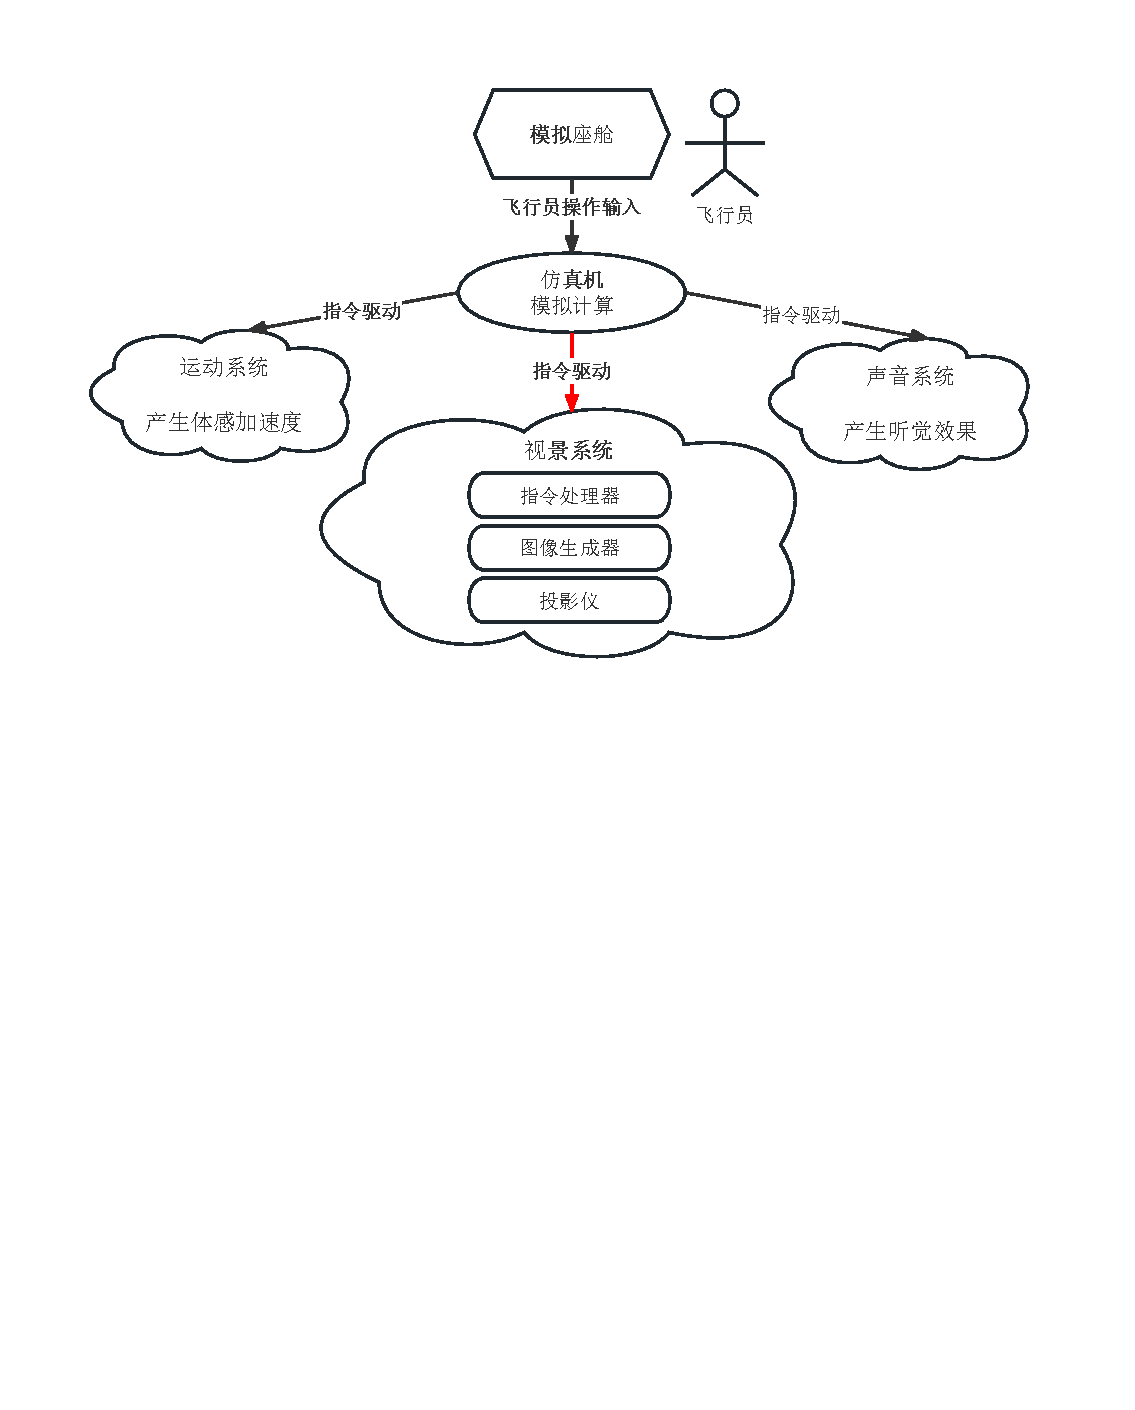
\includegraphics[width=.9\textwidth]{pictures/simstruct.pdf}
        \caption{模拟机运转方式}
        \label{simstruct}
    \end{center}
\end{figure}
\par
由上述可知仿真机是整个FFS的服务端,所有系统都需要与其连接,听从指令才能正常工作。
因此,想要基于仿真机开发视景系统,首先要理解仿真机输出的指令,包括其中的数据组织结构和数字表示方法。
\section{仿真机数据帧分析}
\subsection{数据帧的获取}
对于仿真机于视景系统间行为的分析,最直接的想法是获取处理指令的源代码。经过一番探索,在其中发现了名为Visual Interface进程。但该程序是编译型语言最终得出的二进制指令,并不知道其使用怎样的编译器编译而来;而且此方式通常用于分析主干代码,并不适合获取我们需要的指令细节,这是一条时间成本与预期结果都无法估算的路径。
幸运的是,我们同时拥有一份关于该仿真机的文档,其中含有对于仿真机与视景系统交互指令的详细说明,唯一的问题是该文档编写于20多年前,其时效性有待验证。
\par
有了以上思路后,关于仿真机指令的分析方法就从获取源码变为了验证文档。对于两方通讯方式的研究,网络流量分析也是重要的方法。
为了验证文档内容,我们使用网络抓包工具WireShark截取了运行时仿真机与视景系统交流的原始数据帧,验证数据帧的组织结构与数字表示方法是否与文档相符。图\ref{datastruct}为文档中定义的数据帧结构,抓取到的数据帧如图所示。
\begin{figure}[h!]
    \begin{center}
        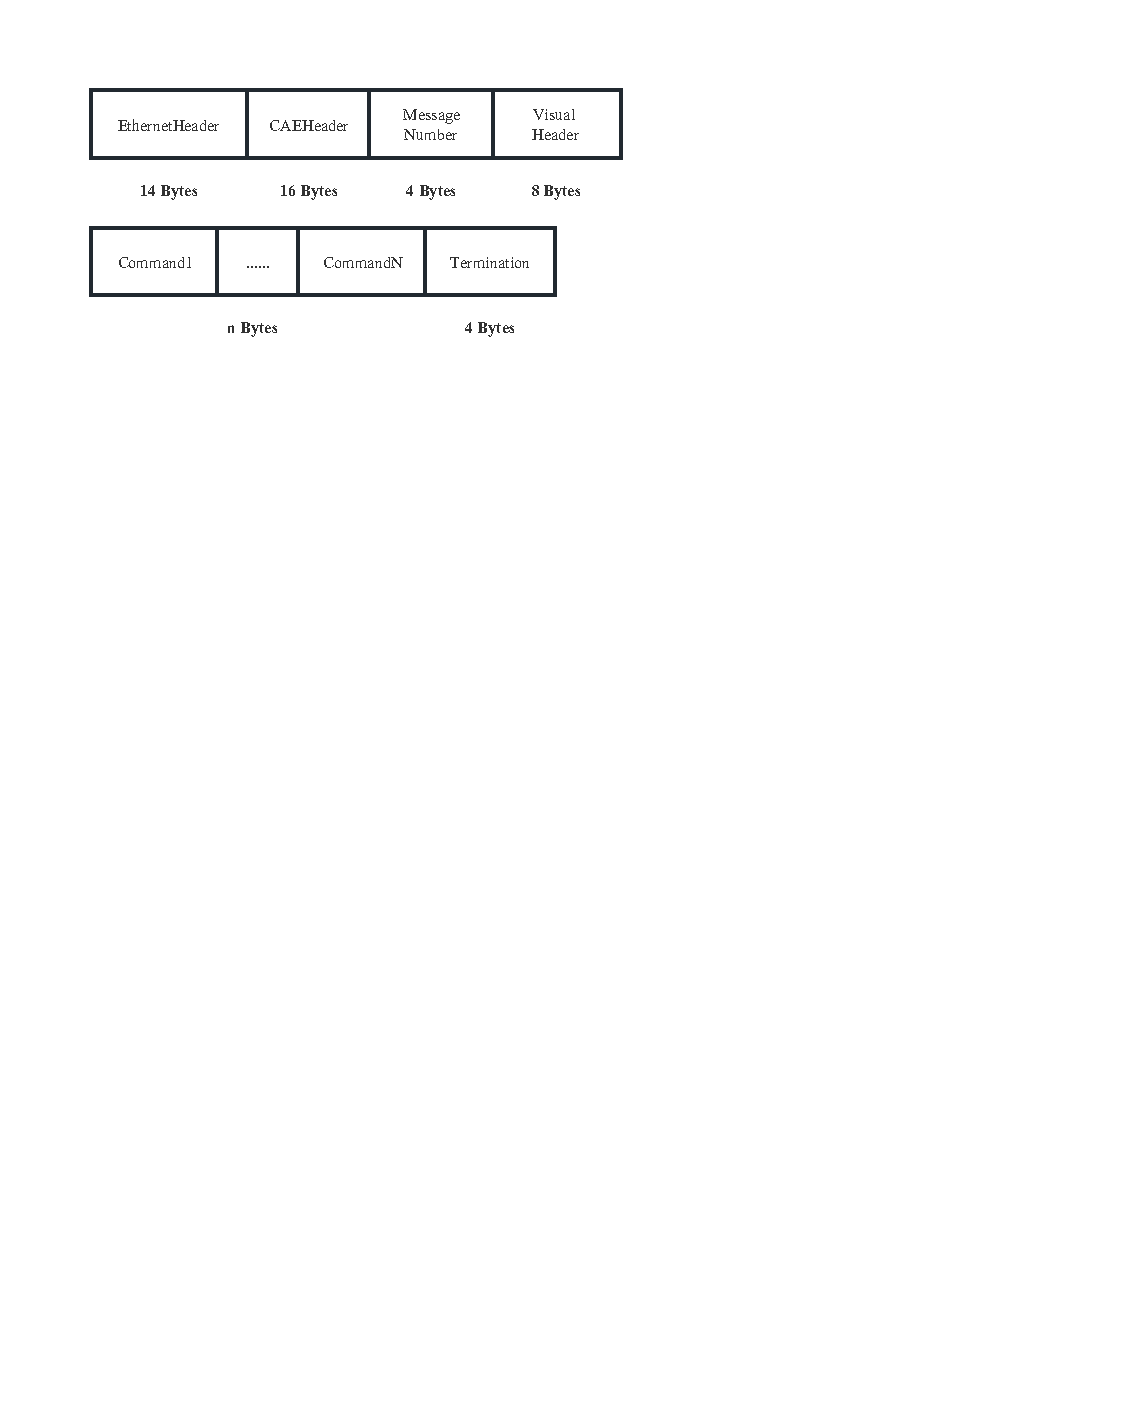
\includegraphics[width=.8\textwidth]{pictures/datastruct.pdf}
        \caption{CAE仿真机数据帧结构}
        \label{datastruct}
    \end{center}
\end{figure}
\subsection{数据帧的解读}
通过对比文档中的数据帧结构说明和截取到的真实数据帧,从该数据帧头部仅有Ethernet Header可以得出仿真机是一个非常底层的设备。从网络模型角度看其最高层是数据链路层,数据内容用以太网协议封装后便进行发送,接收数据也只能仅被以太网协议封装过,否则仿真机无法正确理解反馈信息。因此无法通过工作于传输层以上的传统socket连接模式与本视景系统交流。
图\ref{netlayer}形象的解释了仿真机与视景系统的网络层级差异。
\begin{figure}[h]
    \begin{center}
        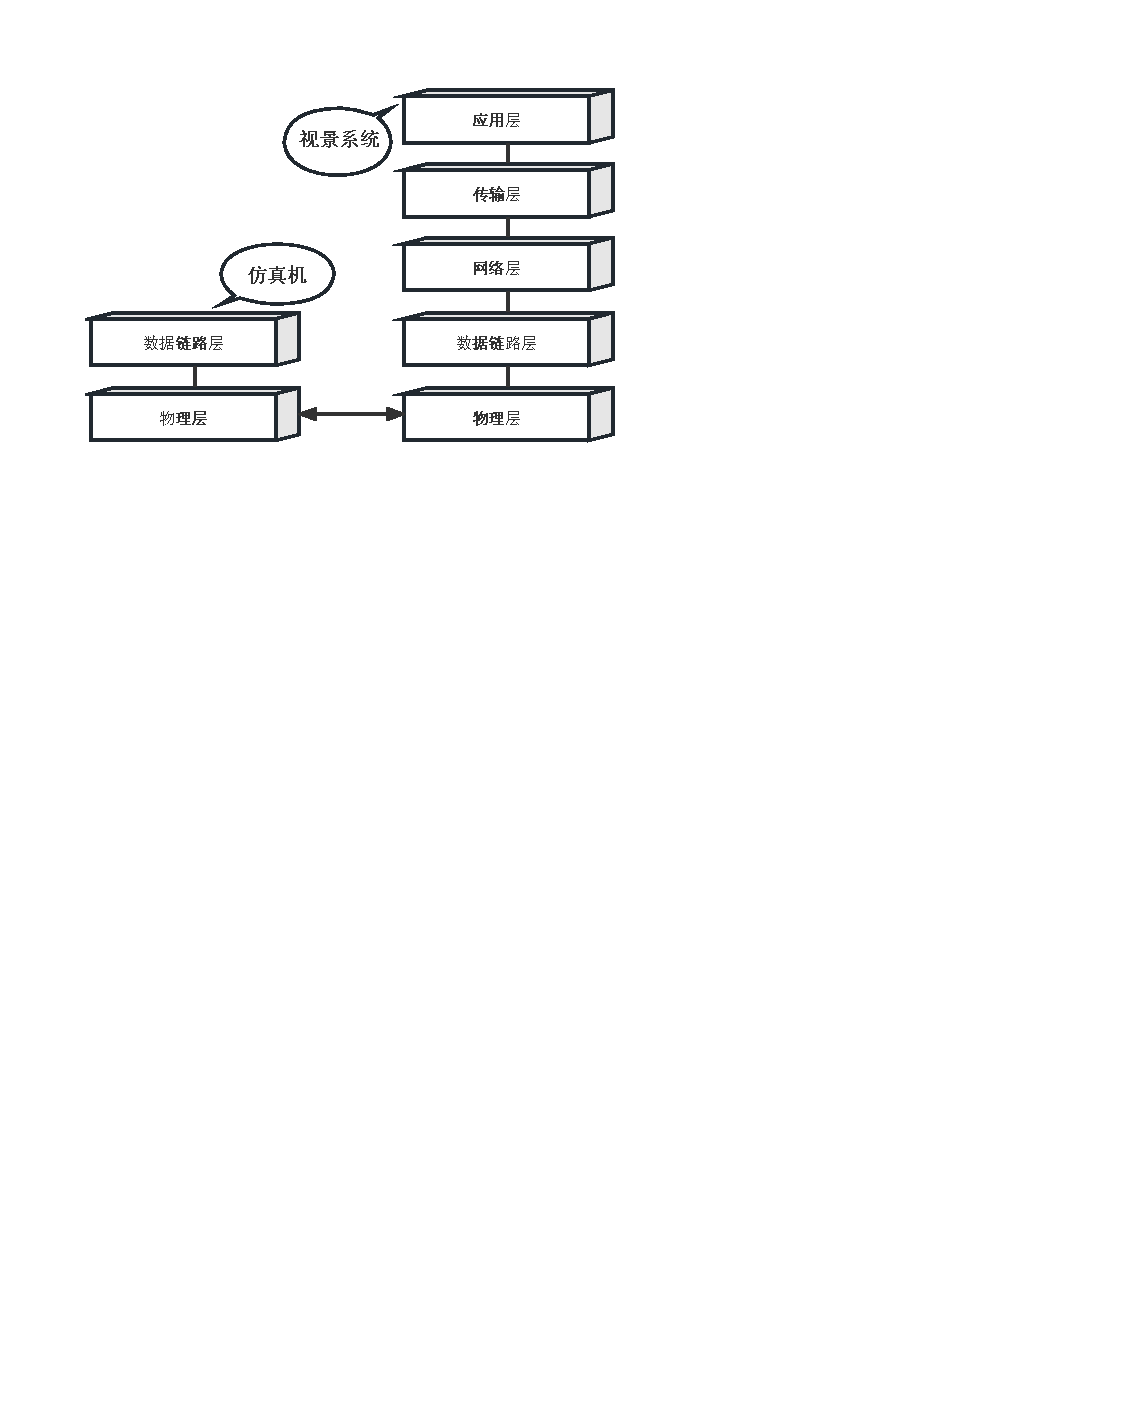
\includegraphics[width=.8\textwidth]{pictures/netlayer.pdf}
        \caption{仿真机与视景系统层级差异}
        \label{netlayer}
    \end{center}
\end{figure}
\par
当剥去数据帧头部的以太网协议头和CAE自定义的部分信息后便余下该数据帧中的所有指令数据,一个数据帧可能包含多条指令。
此处以指令代号为21H的指令为例(H表示十六进制),此指令在飞行模拟中十分关键,其中以经纬度海拔和欧拉角的形式给出了飞机的位置和姿态信息,是仿真机每帧运行都要发出的指令。
文档中关于该指令数据结构的描述如图\ref{21h}中的结构体所示。其种Int32仅代表对应字段占据了32bit,并不表示实际数据类型。由于仿真机侧的数据序列化并没有使用任何数据交换协议,
如果文档内容正确,则可以使用该结构体完成对应数据段的反序列化。
\begin{figure}[h!]
    \centering
     \lstinputlisting[basicstyle= \zihao{-5}]{pictures/21h.txt}
    \caption{21H指令结构}
    \label{21h}
\end{figure}
\par
为了验证文档的时效性,我们需要对该指令中数据的合理性进行检查。在这步工作前需要先进行数字表示方式的转换。
仿真机发送指令中的字段并不是可以直接读取的浮点数,需要做出进一步的转换。对于角度信息一般占32位,其数值单位为$360°/2^{32}$,即一份是一个非常小的角度,可表示范围是-180°到179.999°。
对于海拔这类高度或长度而言,单位统一为0.5mm,即一份为半个毫米。此类数据只需要通过乘法做单位转换。
\par
经纬度这种八字节属性的转换则稍微复杂。其中前四个字节为高位,且前24位表示符号,剩余8位表示高位数字,后四个字节为低位,即单位是$360°/2^{40}$。
且由于补码原因,需要对低位数字进行判断。低位数一定是一个正数,若为负数,则需要按照补码规则转换为正数再与高位相加。图\ref{llconv}中给出了转换经纬度时使用的算法。
$$ffffff80 \qquad 00000000 \qquad represents \qquad -180.00degrees$$
$$00000040 \qquad 00000000 \qquad represents \qquad 90.00 degrees$$

\begin{figure}[h!]
    \centering
     \lstinputlisting[basicstyle= \zihao{-5}]{pictures/llConvert.txt}
    \caption{经纬度数字转换算法}
    \label{llconv}
\end{figure}
\par
当完成数字转换后便可以进行正式的合理性检查,为此我们对本次截取到的六万余条21H指令进行了转换,将其位置在GIS系统中进行标注,最终形成了如图\ref{GIStrace}所示的飞行轨迹。轨迹起始位置精确的位于宝安机场的跑道上,
起飞后环绕深圳市区飞行,最终截止于羊台山森林公园。与飞行员核对后确认本路径准确无误,说明文档对于指令21H的描述完全正确,该指令解读完成。
\begin{figure}[h!]
    \begin{center}
        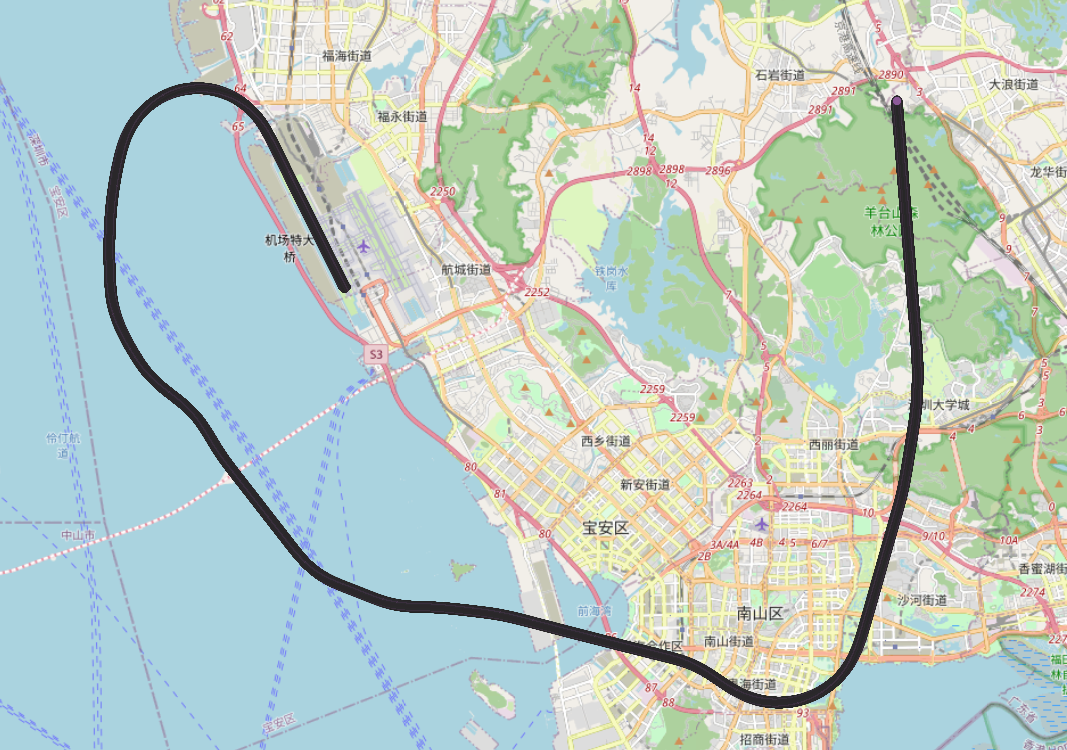
\includegraphics[width=.9\textwidth]{pictures/trace.png}
        \caption{GIS绘制路径}
        \label{GIStrace}
    \end{center}
\end{figure}
\par
目前阶段通过结合已有文档和飞行员经验,已完成21条仿真机控制指令和5条视景系统反馈指令的解读,其中囊括了飞机地理位置、机身灯光、雨雪天气、能见度等指令,也包含了如碰撞反馈等逆向的指令。保障视景系统中如飞行、天气变化、碰撞检测等基本功能的实现。
表\ref{caecommand}列举了已成功验证的部分仿真机指令代号及功能。
\begin{table}[h!]
    \begin{center}
        \caption{仿真机部分指令列表}
        \label{caecommand}
        \renewcommand\arraystretch{1.5}
        \begin{tabularx}{0.8\textwidth}{ 
            | >{\centering\arraybackslash\hsize=.15\hsize\linewidth=\hsize}X 
            | >{\raggedright\arraybackslash\hsize=.85\hsize\linewidth=\hsize}X 
            | }
            \hline
            \textbf{代号} & \textbf{指令用途}\\
            \hline
            21H &  负责控制飞机的位置与飞行姿态,是仿真机每帧都要更新的最基本指令,其通过经纬度海拔确定位置,通过该位置东北天坐标系下的欧拉角确定姿态。\\
            \hline
            42H &  负责控制机身主要位置灯光开关和照明角度,指令中包含灯光的状态和相对机身水平竖直方向的两个角度。\\
            \hline
            43H &  负责控制机场灯光,指令中包括跑道滑行灯、PAPI灯、四组不同距离的环境灯等灯光的状态。\\
            \hline
            44H &  负责部分天气效果的控制,指令中包含下雨、下雪及其程度的描述,云层的效果等信息。\\
            \hline
            45H &  负责能见度的控制,指令中包含雾的浓度,可视角度等信息,在盲降训练时会被使用。\\
            \hline
            47H &  负责所处时间段的控制,指令中包含白昼、黑夜、黎明、黄昏四种时间段信息,且根据不同的日期会有不同的月相信息。反映到视景系统中会产生不同的天光。\\
            \hline
            86H &  负责一些通用信息的反馈,包括视景中使用的地球坐标系类型,当前加载的机场编号,是否发生严重碰撞等等。\\
            \hline
            82H &  负责反馈飞机上某点的离地高度,一般是用于降落是起落架相关信息的计算。\\
            \hline
        \end{tabularx}
    \end{center}
\end{table}
% \section{视景系统整体概述}
% 视景系统是FFS中负责连续生成模拟座舱前方飞行画面的系统。飞行员在模拟座舱中的操作将作为仿真机的输入,经过模拟计算后输出如位置、姿态、灯光等一系列指令,图像生成器根据指令要求执行逻辑后便可渲染连贯的飞行画面,提供模拟飞行的视觉效果。
% 同时图像生成器也要以指令的形式反馈给仿真机如碰撞等信息。仿真机可以据此通知如声音、运动系统做出相应反馈。
% \par
% 由上述可知仿真机相当于FFS的服务端,视景系统类似客户端,但此案例的服务端与客户端在网络体系结构中处于不同层级,需要请一个翻译才能正常进行数据交换,本系统中将该翻译角色称为虚拟仿真机。
% 视景系统整体架构如图\ref{framework}所示。仿真机作为一个底层网络设备,其只能接收或发送仅用以太网协议封装的数据包,且使用该公司自定义的数据交换协议;虚拟仿真机作为翻译需要对双方的消息解封、转换再封装,最后发送。同时在没有仿真机的开发环境下也可以读取模拟数据实现流程;
% 虚拟仿真机与客户端之间使用ProtoBuffer作为数据交换协议,TCP通信任务由Tbuspp插件承担。图像生成器需要根据收到的指令先完成数据同步工作,再执行逻辑,计算反馈信息。图中虚线框中的部分包含了数据由仿真机到图像生成器中被使用,生成的反馈信息再最终回到仿真机的全过程,此部分便是视景系统中的数据交换子系统。
% \par
% 图像生成器中还含有许多重要的功能组成部分。首先引擎核心为其提供了渲染、物理、脚本、数学计算等运行核心组件,许多逻辑依赖其中的方法实现,逻辑执行结束后也需要渲染介入。
% 机场资产则是场景的数据库,地形、建筑、纹理等资源皆存于其中,需要根据飞机所处位置去查找并加载这些资源,这对于数据的组织形式,查找策略都有较高的要求。
% 投影同步插件负责在FFS上运行时控制多台投影仪投影相同的一帧以减少画面撕裂,另外由于模拟座舱前方是一个球幕,需要校准球幕投影时发生的畸变。




\section{数据交换子系统需求分析}
确定了仿真机与原配视景系统间的指令沟通方式后,便可以开展数据交换子系统的设计与实现工作。系统设计的第一步是需求分析,其主要目的是明晰非形式化
的需求,最终产生完整的需求规格说明。本节首先分析了系统中的涉众,阐述了涉众对系统的期望。
随后从系统的角度解释软件,定义了系统的功能性需求和非功能性需求。
最后在明确需求的基础上,将各需求拆解为用例,使用4+1视图确定了系统的整体结构。
\subsection{涉众分析}
本系统作为视景系统中负责数据交换的子系统,负责连接双方并转换指令的角色称为虚拟仿真机,而负责根据收到的指令执行逻辑并完成渲染的角色称为图像生成器。
虚拟仿真机作为桥梁希望与仿真机和图像生成器双向交流,而图像生成器希望以稳定的数据驱动逻辑运行。
详细的涉众分析如表\ref{stakeholder}所示。
\begin{table}[h!]
    \begin{center}
        \caption{涉众分析列表}
        \label{stakeholder}
        \renewcommand\arraystretch{1.5}
        \begin{tabularx}{\textwidth}{ 
            | >{\centering\arraybackslash\hsize=.25\hsize\linewidth=\hsize}X 
            | >{\raggedright\arraybackslash\hsize=.75\hsize\linewidth=\hsize}X 
            | }
            \hline
            \textbf{涉众名称} & \textbf{涉众期望}\\
            \hline
            虚拟仿真机 &  虚拟仿真机作为仿真机与图像生成器间的桥梁,虚拟仿真机希望能正确解释并转换双发发送的指令,
                         能按照仿真机的运行频率及时读取数据并及时发送给图像生成器。同时作为视景系统的一部分,能够屏蔽不同仿真机数据组织结构的差异。\\
            \hline
            图像生成器 &  图像生成器作为执行逻辑和渲染画面的角色,希望从虚拟仿真机处取得指令数据包,并分割为一条条单一指令供对应逻辑运行。\\
            \hline
        \end{tabularx}
    \end{center}
\end{table}
\subsection{功能性需求}
图像生成器依据仿真机指令进行飞行画面渲染并反馈飞行数据要求仿真机与图像生成器之间进行双向数据交换。上一节中对仿真机的分析里提到,仿真机作为底层设备其输出与输入均为只用以太网协议封装的数据帧,这种数据帧不能交由网络协议栈处理,
虚拟仿真机应该自己实现解封和封装过程,转换为自定义指令后的数据则可以通过TCP协议栈发送给图像生成器。虚拟仿真机同时承担着在没有仿真机的开发条件下读取模拟数据帧驱动视景运转的责任。

% 在信息的传输过程中避免不了存在网络波动;且虚拟仿真机与图像生成器间用无法广播的TCP协议通信,对于单一图像生成器而言数据到达频率可能不稳定,对于多个图像生成器而言同一数据到达时刻也不相同。
% 因此需要进行数据同步抵消差异。另外从单一图像生成器角度,逻辑帧的开始时间受渲染帧约束,不能保证绝对稳定,如果按照仿真机的原始数据飞行可能会产生不自然的闯动,需要一定的数据平滑策略减少影响。
在本视景系统中具体得到数据流动可用下面这一完整流程描述:
\begin{itemize}
    \item [(1)]
    仿真机根据飞行员的输入计算飞行状态,产生一条条指令数据,将这些指令数据仅通过以太网协议封装后以数据链路层数据帧的形式输出。
    \item [(2)]
    虚拟仿真机接收数据链路层数据帧,去除以太网协议的头尾内容,完成解封。识别指令代号后,直接使用对应结构体反序列化指令内容。
    \item [(3)]
    将指令中特殊数字表示方式下的数据通过算法转换为便于图像生成器使用的数字形式。如将经度0000007f ffffffff转换为179.99后,结合纬度和海拔信息转换为笛卡尔坐标系位置,再赋值给自定义指令中的对应字段,生成我们自定义的指令集。
    \item [(4)]
    将该结构化数据通过ProtoBuffer协议进行序列化,并通过TCP协议发送给图像生成器,此过程中的协议封装则全权交由操作系统的内核网络协议栈完成。
    \item [(5)]
    图像生成器接收到数据后,同样由内核网络协议栈解封,再通过ProtoBuffer协议进行反序列化得到指令结构化数据,供给逻辑线程使用。
    \item [(6)]
    逻辑线程的反馈信息则通过完全相反的过程,最终逆向发送到仿真机。
\end{itemize}


\par
% 另外数据交换子系统作为视景系统的一部分,流经它的数据最终要服务于视景系统中的部分逻辑,且反馈数据也来自于逻辑执行。
% 但项目初始阶段视景系统中并不存在任何运行逻辑,因此我们将飞行模拟最基础的飞机飞行一系列逻辑作为数据交换子系统的部分功能。它将使用接收到的指令完成飞行,并将检测到的地形信息作为反馈。
% 最终飞行画面是否正确、流畅也是判断数据交换子系统是否正常运作的重要依据。
整个指令数据传输的过程中需要保证虚拟仿真机与图像生成器依照仿真机的工作频率运行,即数据到达便要处理并发送,这个过程中有一些缓存机制需要禁用。
数据交换子系统的功能性需求列表如表\ref{funcreq}所示。
\begin{table}[h!]
    \begin{center}
        \caption{系统功能性需求列表}
        \label{funcreq}
        \renewcommand\arraystretch{1.5}
        \begin{tabularx}{\textwidth}{ 
            | >{\centering\arraybackslash\hsize=.1\hsize\linewidth=\hsize}X 
            | >{\centering\arraybackslash\hsize=.3\hsize\linewidth=\hsize}X 
            | >{\raggedright\arraybackslash\hsize=.6\hsize\linewidth=\hsize}X 
            | }
            \hline
            \textbf{ID} & \textbf{需求名称} & \textbf{需求描述}\\
            \hline
            R1 & 与仿真机交互 & 虚拟仿真机可以绕过所在操作系统的网络协议栈,直接读取或生成流经网卡的原始数据帧,需要亲自实现解封和封装数据帧的过程。
                               此过程中需要按照仿真机的频率读取网卡数据,确保指令数据的实时性。\\
            \hline
            R2 & 指令数据转换 & 虚拟仿真机可以将仿真机使用的指令与图像生成器中使用的指令进行映射,同时需要进行数字表示方法的转换,方便双方对于指令数据的使用。\\
            \hline 
            R3 & 与图像生成器交互 & 虚拟仿真机可以与图像生成器进行自定义指令的交互,需要对被拆分处理的多条指令重新粘合发送,收发的过程中使用高效的数据交换协议对指令内容序列化和反序列化。\\
            % \hline 
            % R4 & 数据同步与平滑 & 图像生成器不可以立即使用到达的数据指令,存储几帧内容与其他机器进行同步处理。图像生成器可以对存储的内容进行平滑,减少逻辑帧的不稳定带来的抖动。\\
            \hline
        \end{tabularx}
    \end{center}
\end{table}


\subsection{非功能性需求}
帧率是动态画面视觉体验的重要因素,对于电视与电影这类视频行业来讲24Hz以上的帧率便能达到良好的观看体验\cite{frame}。但对于需要飞行员实施操控的飞行模拟而言,60Hz以上的帧率才不会让飞行员产生操作延迟的感觉,因此本视景系统初期要求在训练基地的FFS设备上能达到60Hz的帧率,且运行时不出现可观察到的抖动现象。
目前国内的进口模拟机来自CAE等外国公司,虽然各厂商的仿真机都是数据链路层设备,但他们的指令有不同的数据组织结构和数字表示方法,数据交换子系统需要屏蔽这些差异,方便日后的二次开发以适配不同仿真机。系统的非功能性需求列表如表\ref{unfuncreq}所示。
\begin{table}[h!]
    \begin{center}
        \caption{系统非功能性需求列表}
        \label{unfuncreq}
        \renewcommand\arraystretch{1.5}
        \begin{tabularx}{\textwidth}{ 
            | >{\centering\arraybackslash\hsize=.1\hsize\linewidth=\hsize}X 
            | >{\centering\arraybackslash\hsize=.3\hsize\linewidth=\hsize}X 
            | >{\raggedright\arraybackslash\hsize=.6\hsize\linewidth=\hsize}X 
            | }
            \hline
            \textbf{ID} & \textbf{需求名称} & \textbf{需求描述}\\
            \hline
            R1 & 运行帧率 & 飞行画面在60Hz以上才不会产生明显操作延迟感,因此要求初期在真实FFS设备上能够达到最低60Hz的渲染帧率,也意味着数据交换子系统能够以这个频率处理数据。且日后经游戏引擎角度的不断优化能够达到100Hz以上。\\
            \hline
            R2 & 可靠性 & 一节飞行训练课约为50分钟,要求视景系统在连续运行50分钟期间不出现明显的画面撕裂、抖动和帧率下降趋势。\\
            \hline
            R3 & 可扩展性 & 由于国内现存各厂商的仿真机均使用自定义数据组织结构和数字表示方法,数据交换子系统应体现仿真机侧无关性,将不同厂商的指令映射为我们自定义的指令集,方便经过二次开发后在各类仿真机上搭载。\\
            \hline
        \end{tabularx}
    \end{center}
\end{table}

\subsection{用例设计}

\begin{figure}[h]
    \begin{center}
        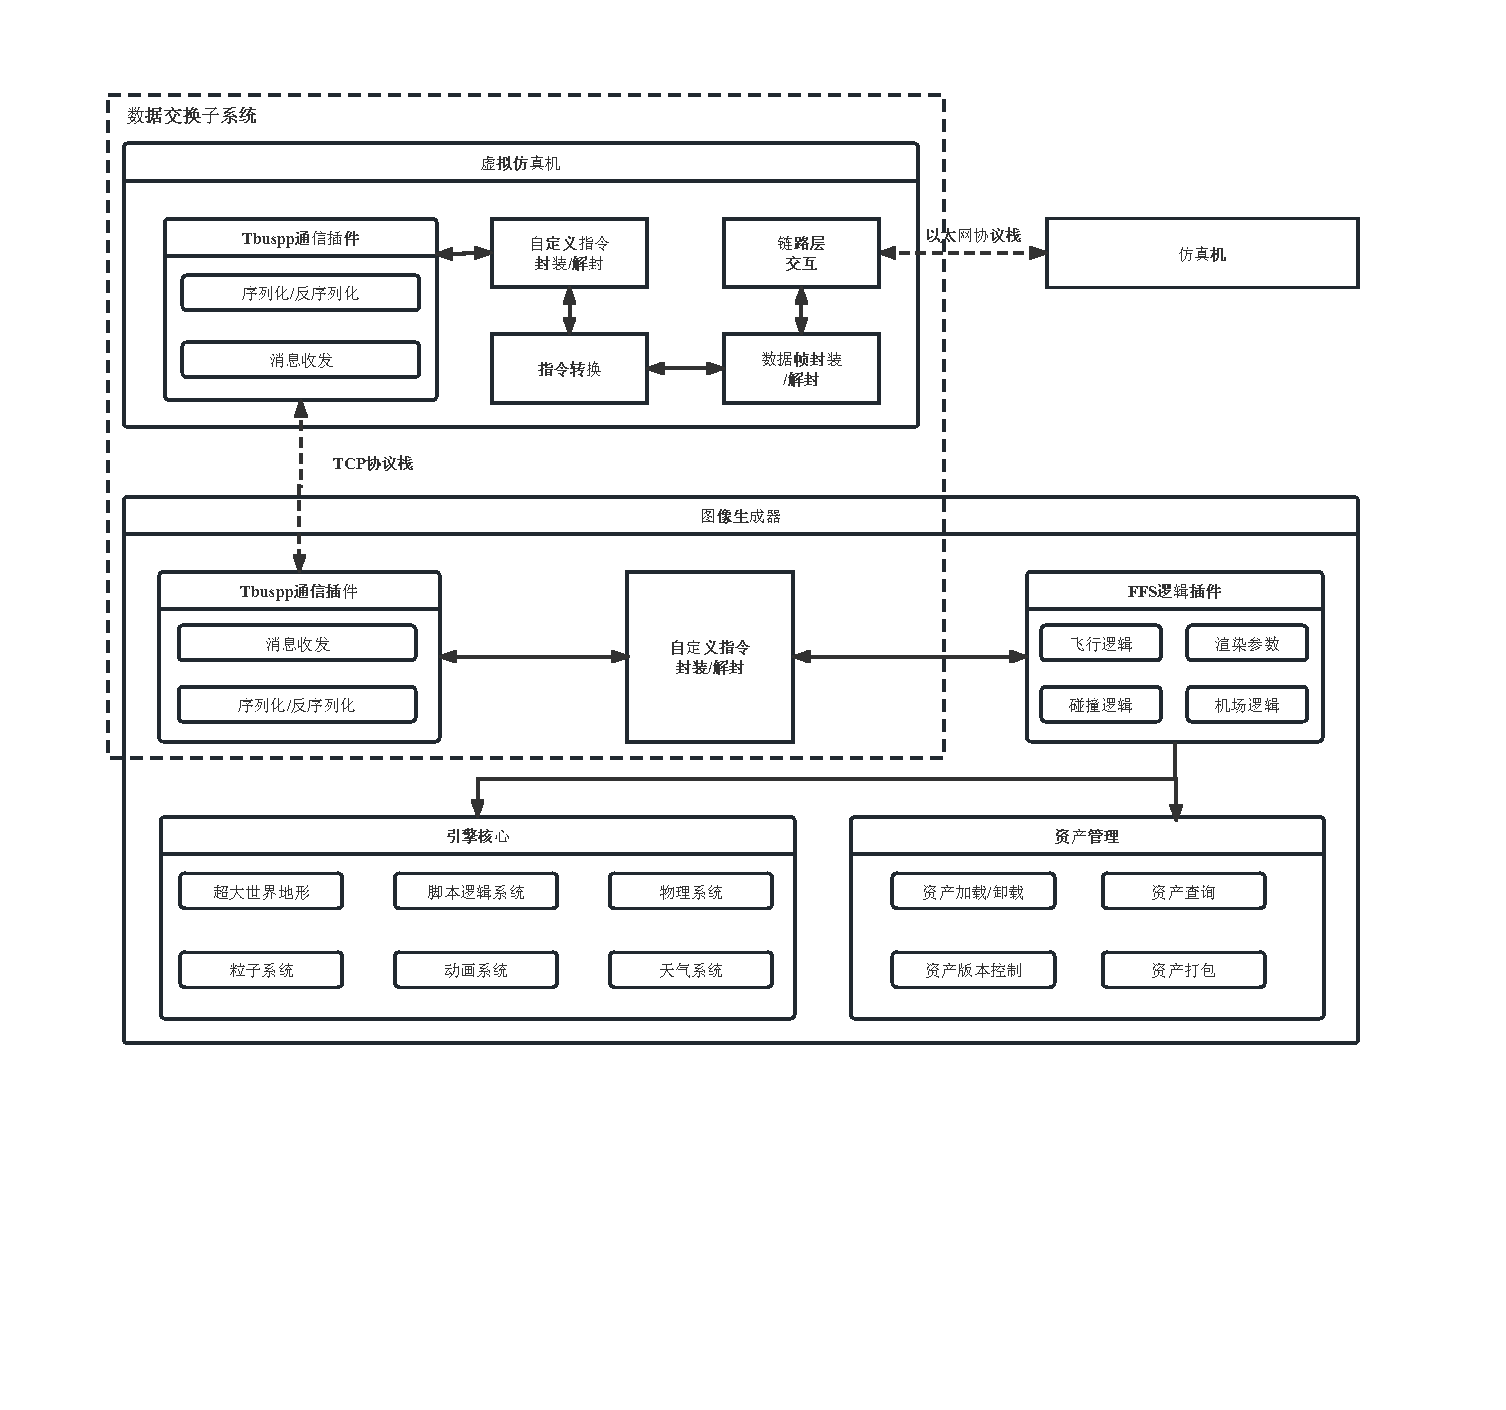
\includegraphics[width=\textwidth]{pictures/sysedge.pdf}
        \caption{数据交换子系统边界}
        \label{framework}
    \end{center}
\end{figure}
经过需求分析后最终确定将数据交换子系统划分为十个用例,系统用例图如图\ref{usecase}所示。其中的角色分为虚拟仿真机,客户端和开发人员。
虚拟仿真机与仿真机建立数据链路层连接,并通过仅用以太网协议封装的数据帧交互。虚拟仿真机中的指令数据经过解封、转换、包装等一系列动作后成为一组自定义指令,序列化后通过Tbuspp发送给客户端;
客户端接收数据后,根据反序列化后得到的指令内容执行逻辑,逻辑执行的结果最终用于加载对应资源和渲染画面等过程。
飞行中产生的反馈信息则由客户端逆向发送最终以数据帧形式给到仿真机。作为开发人员在测试过程中可以切换不同的视角观察飞机和场景的状态,及时对问题做出调整。
\par
具体而言,虚拟仿真机的用例包括建立链路层连接、收取数据帧、发送数据帧、读取模拟数据、仿真机指令转自定义指令、自定义指令转仿真机指令和收发TCP消息。
客户端的用例包括收发TCP消息、飞行控制、检测地形信息。开发人员的用例包括切换摄像机视角。总共十个用例。

\begin{figure}[h!]
    \begin{center}
        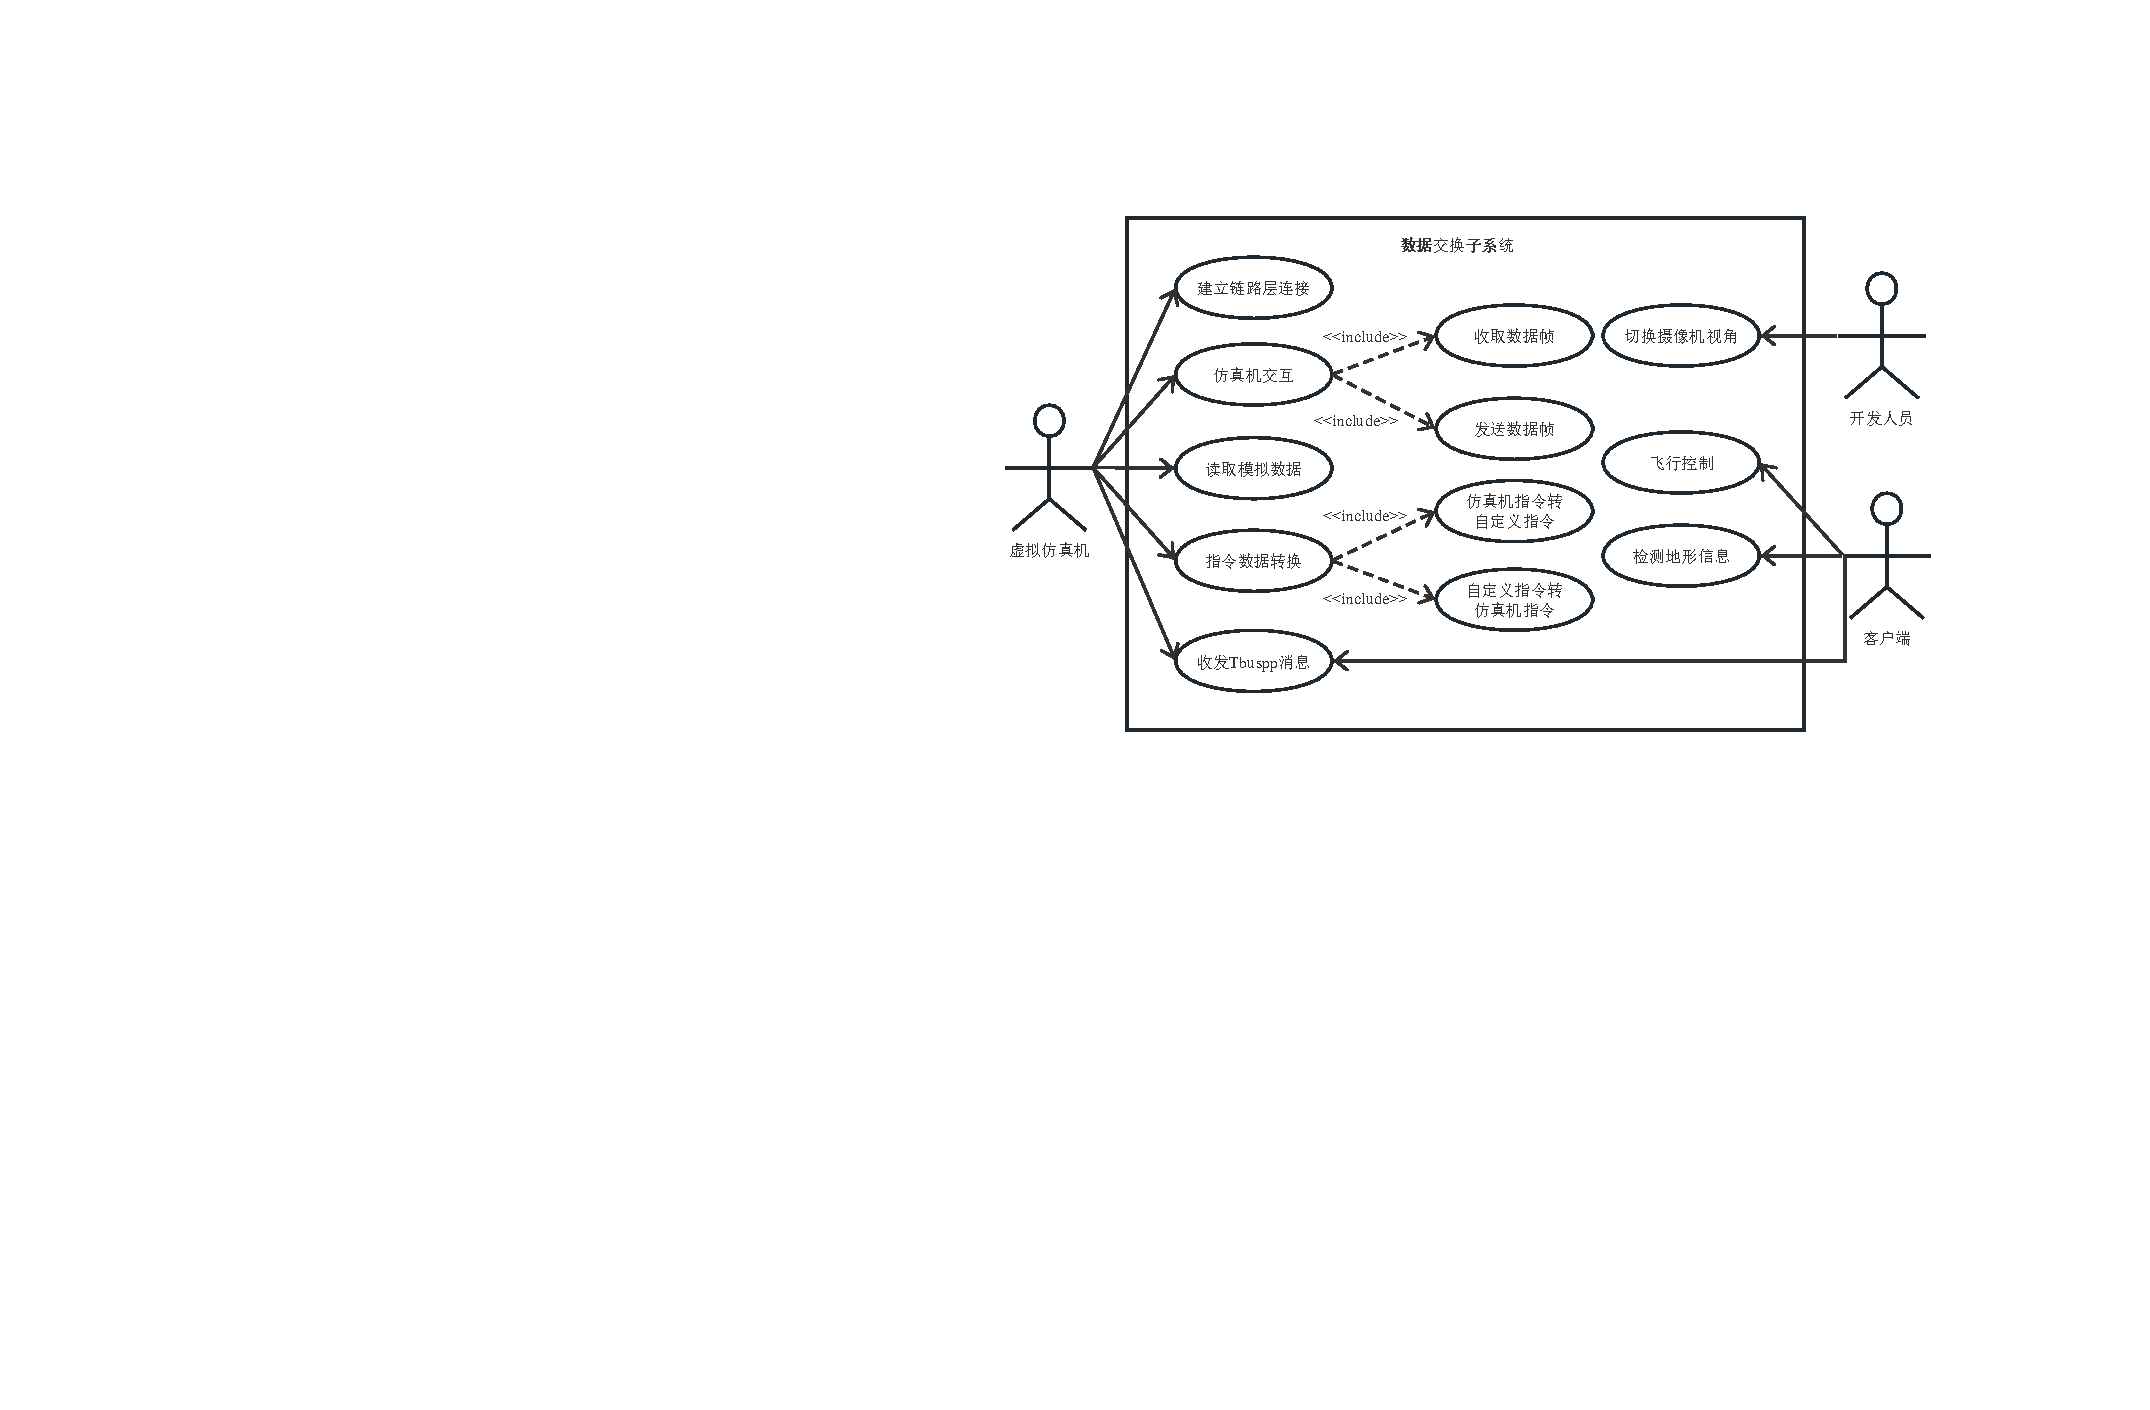
\includegraphics[width=\textwidth]{pictures/usecase.pdf}
        \caption{数据交换子系统用例图}
        \label{usecase}
    \end{center}
\end{figure}

\par
下面将对用例图中提到的系统用例通过用例描述表的形式进行详细解释。
\par
建立链路层连接,是虚拟仿真机与仿真机建立沟通路径的方式。如图\ref{datastruct}中的CAE仿真机数据帧结构所示,由于仿真机是底层设备,其产生的数据帧不含有IP头、TCP头等信息,
所以不能直接交由虚拟仿真机运行环境中的网络协议栈处理,必须由虚拟仿真机亲自侦听网卡上的原始数据帧,并亲自解封或封装。用例的具体情况如表\ref{usecase1}所示。

\begin{table}[htbp]
    \begin{center}
        \caption{建立链路层连接用例描述表}
        \label{usecase1}
        \renewcommand\arraystretch{1.5}
        \begin{tabularx}{0.8\textwidth}{ 
            | >{\centering\arraybackslash\hsize=.5\hsize\linewidth=\hsize}X 
            | >{\raggedright\arraybackslash\hsize=1.5\hsize\linewidth=\hsize}X 
            | }
            \hline
            \textbf{ID} & \textbf{UC1}\\
            \hline
            参与者 & 虚拟仿真机\\
            \hline
            触发条件 & 视景系统开始运行。\\
            \hline
            前置条件 & 1.虚拟仿真机处于接收仿真机消息模式。\par2.仿真机处于开启状态。\\
            \hline
            后置条件 & 能够与仿真机进行数据交流。\\
            \hline
            优先级 & 高\\
            \hline
            正常流程 &  1.查找运行环境下的网络适配器列表。\par 2.选择其中一个网络适配器。\par 3.获取混杂模式数据包捕获句柄。\par 4. 开启及时转发模式。\\
            \hline
            扩展流程 & 网络适配器不能正常运作,打印错误提示。\\
            \hline
        \end{tabularx}
    \end{center}
\end{table}
\par
收取数据帧,是虚拟仿真机从网卡上读取仿真机发送的数据帧的过程。此过程不依靠网络协议栈自动解封,而是自己实现解封过程。收取具体情况如表\ref{usecase2}所示。
\begin{table}[htbp]
    \begin{center}
        \caption{收取数据帧用例描述表}
        \label{usecase2}
        \renewcommand\arraystretch{1.5}
        \begin{tabularx}{0.8\textwidth}{ 
            | >{\centering\arraybackslash\hsize=.5\hsize\linewidth=\hsize}X 
            | >{\raggedright\arraybackslash\hsize=1.5\hsize\linewidth=\hsize}X 
            | }
            \hline
            \textbf{ID} & \textbf{UC2}\\
            \hline
            参与者 & 虚拟仿真机\\
            \hline
            触发条件 & 仿真机向视景系统发送数据帧。\\
            \hline
            前置条件 & 虚拟仿真机侦听了正确的网卡。\\
            \hline
            后置条件 & 数据帧被分为一个个指令段。\\
            \hline
            优先级 & 高\\
            \hline
            正常流程 & 1.去除数据帧头部信息。\par 2.读取指令长度并按该长度截取。\par 3.将数据段加入指令集合。\par 4.回到流程2循环至全部数据读取结束。\\
            \hline
            扩展流程 & 无\\
            \hline
        \end{tabularx}
    \end{center}
\end{table}
\par
发送数据帧,是虚拟仿真机发送信息到仿真机的过程,此过程同样不依靠网络协议栈自动封装,而是自己实现封装过程。具体情况如表\ref{usecase3}所示。
\begin{table}[htbp]
    \begin{center}
        \caption{发送数据帧用例描述表}
        \label{usecase3}
        \renewcommand\arraystretch{1.5}
        \begin{tabularx}{0.8\textwidth}{ 
            | >{\centering\arraybackslash\hsize=.5\hsize\linewidth=\hsize}X 
            | >{\raggedright\arraybackslash\hsize=1.5\hsize\linewidth=\hsize}X 
            | }
            \hline
            \textbf{ID} & \textbf{UC3}\\
            \hline
            参与者 & 虚拟仿真机\\
            \hline
            触发条件 & 反馈指令到达。\\
            \hline
            前置条件 & 虚拟仿真机侦听了正确的网卡。\\
            \hline
            后置条件 & 仿真机收到视景系统反馈并通知其它系统协同。\\
            \hline
            优先级 & 高\\
            \hline
            正常流程 & 1.反馈指令数据段到达。\par 2.将多条指令按规则粘合在一个数据包中。\par 3.为数据包添加以太网头尾信息。\par 4.将数据帧加入发送队列中。\\
            \hline
            扩展流程 & 无。\\
            \hline
        \end{tabularx}
    \end{center}
\end{table}
\par
国内的FFS全部位于航空公司的训练基地内,其价格昂贵且巨大,无法搬运至开发环境中。在日常开发中,虚拟模拟机需要读取文件中的模拟数据来驱动视景系统运作。具体情况如表\ref{usecase4}所示。
\begin{table}[htbp]
    \begin{center}
        \caption{读取模拟数据用例描述表}
        \label{usecase4}
        \renewcommand\arraystretch{1.5}
        \begin{tabularx}{0.8\textwidth}{ 
            | >{\centering\arraybackslash\hsize=.5\hsize\linewidth=\hsize}X 
            | >{\raggedright\arraybackslash\hsize=1.5\hsize\linewidth=\hsize}X 
            | }
            \hline
            \textbf{ID} & \textbf{UC4}\\
            \hline
            参与者 & 虚拟仿真机\\
            \hline
            触发条件 & 使用模拟数据驱动视景系统运作。\\
            \hline
            前置条件 & 虚拟仿真机处于读取模拟数据模式。\\
            \hline
            后置条件 & 文本信息被转化为数据帧信息。\\
            \hline
            优先级 & 高\\
            \hline
            正常流程 & 1.指定文件路径。\par 2.按行读取文本。\par 3.将16进制字符两两一组转换为一个字节。\par 4.按用例二中的流程进行。\\
            \hline
            扩展流程 & 文件不存在或格式有错误则产生警告。\\
            \hline
        \end{tabularx}
    \end{center}
\end{table}

\par
仿真机指令转自定义指令,是虚拟仿真机将难以理解的仿真机指令转换为可供视景系统使用的子定义指令的过程。具体情况如表\ref{usecase5}所示。
\begin{table}[htbp]
    \begin{center}
        \caption{仿真机指令转自定义指令用例描述表}
        \label{usecase5}
        \renewcommand\arraystretch{1.5}
        \begin{tabularx}{0.8\textwidth}{ 
            | >{\centering\arraybackslash\hsize=.5\hsize\linewidth=\hsize}X 
            | >{\raggedright\arraybackslash\hsize=1.5\hsize\linewidth=\hsize}X 
            | }
            \hline
            \textbf{ID} & \textbf{UC5}\\
            \hline
            参与者 & 虚拟仿真机\\
            \hline
            触发条件 & 存在待转换的仿真机指令。\\
            \hline
            前置条件 & 定义了对应仿真机指令的自定义指令。\\
            \hline
            后置条件 & 构建了一个自定义指令。\\
            \hline
            优先级 & 高\\
            \hline
            正常流程 & 1.获取仿真机指令中的指令代号。\par 2.根据指令代号查找对应的转换器。\par 3.使用转换器完成转换。\\
            \hline
            扩展流程 & 对于暂时使用不到的仿真机指令直接丢弃。\\
            \hline
        \end{tabularx}
    \end{center}
\end{table}

\par
自定义指令转仿真机指令,是反馈信息时虚拟仿真机将自定义指令翻译为仿真机使用的仿真机指令的过程。具体情况如表\ref{usecase6}所示。
\begin{table}[htbp]
    \begin{center}
        \caption{自定义指令转仿真机指令用例描述表}
        \label{usecase6}
        \renewcommand\arraystretch{1.5}
        \begin{tabularx}{0.8\textwidth}{ 
            | >{\centering\arraybackslash\hsize=.5\hsize\linewidth=\hsize}X 
            | >{\raggedright\arraybackslash\hsize=1.5\hsize\linewidth=\hsize}X 
            | }
            \hline
            \textbf{ID} & \textbf{UC6}\\
            \hline
            参与者 & 虚拟仿真机\\
            \hline
            触发条件 &  存在待转换的自定义指令。\\
            \hline
            前置条件 & 无\\
            \hline
            后置条件 & 构建了一个仿真机指令。\\
            \hline
            优先级 & 高\\
            \hline
            正常流程 & 1.获取自定义指令的指令代号。\par 2.根据指令代号查找对应的转换器。\par 3.使用转换器完成转换。\\
            \hline
            扩展流程 & 无\\
            \hline
        \end{tabularx}
    \end{center}
\end{table}
\par
视景系统与虚拟仿真机利用Tbuspp插件进行沟通,双方都需要对Tbuspp消息进行收发。具体情况如表\ref{usecase7}所示。
\begin{table}[htbp]
    \begin{center}
        \caption{收发Tbuspp消息用例描述表}
        \label{usecase7}
        \renewcommand\arraystretch{1.5}
        \begin{tabularx}{0.8\textwidth}{ 
            | >{\centering\arraybackslash\hsize=.5\hsize\linewidth=\hsize}X 
            | >{\raggedright\arraybackslash\hsize=1.5\hsize\linewidth=\hsize}X 
            | }
            \hline
            \textbf{ID} & \textbf{UC7}\\
            \hline
            参与者 & 虚拟仿真机\&客户端\\
            \hline
            触发条件 & 有自定义指令待发送。\\
            \hline
            前置条件 & 双方使用Tbuspp成功建立连接。\\
            \hline
            后置条件 & 无\\
            \hline
            优先级 & 高\\
            \hline
            正常流程 &  数据发送过程:\par 1.用ProtoBuffer协议序列化自定义指令结构。\par 2.将消息写入Tbuspp发送队列。\par 
                       数据接收过程:\par 1.从Tbuspp接收队列读取数据。\par 2.使用ProtoBuffer协议反序列化消息得到自定义指令结构。\\
            \hline
            扩展流程 & 无\\
            \hline
        \end{tabularx}
    \end{center}
\end{table}

\par
视景系统中的飞机需要按照收到的飞行状态在地心地固坐标系下的场景进行运动,主要使用飞机的位置和旋转信息,根据飞行画面可以证明数据交换系统的功能是否正常。具体情况如表\ref{usecase7}所示。
\begin{table}[htbp]
    \begin{center}
        \caption{飞行控制用例描述表}
        \label{usecase8}
        \renewcommand\arraystretch{1.5}
        \begin{tabularx}{0.8\textwidth}{ 
            | >{\centering\arraybackslash\hsize=.5\hsize\linewidth=\hsize}X 
            | >{\raggedright\arraybackslash\hsize=1.5\hsize\linewidth=\hsize}X 
            | }
            \hline
            \textbf{ID} & \textbf{UC8}\\
            \hline
            参与者 & 客户端\\
            \hline
            触发条件 & 客户端收到飞机飞行相关指令数据。\\
            \hline
            前置条件 & 存在飞机实体及对应位置场景资源。\\
            \hline
            后置条件 & 连续更新飞机位置和姿态获得动态视景效果。\\
            \hline
            优先级 & 高\\
            \hline
            正常流程 & 1.获取经纬度海拔和欧拉角信息。\par 2.将LLA坐标转换为ECEF坐标。\par 3.将飞机模型置于场景中该坐标位置。\par 4.根据欧拉角调整飞机姿态。\\
            \hline
            扩展流程 & 无\\
            \hline
        \end{tabularx}
    \end{center}
\end{table}




\section{数据交换子系统概要设计}
数据交换子系统的架构设计如图\ref{subframe}所示,整个系统分为三个部分,仿真机与虚拟仿真机间通过数据帧进行交互,虚拟仿真机与游戏引擎通过TCP协议交互。
仿真机的作用是对飞行员的操作输入进行仿真计算,得出飞机状态,这部分由FFS厂商设计开发。虚拟仿真机则将不同的仿真机数据协议翻译为统一的供视景系统使用的指令结构体,以此屏蔽仿真机的差异。
游戏引擎的只需按照收到的指令数据渲染飞行画面,并提供简单的反馈信息。
\par 
在数据交换子系统中虚拟仿真机的通信服务完全使用C++语言开发,游戏引擎中核心功能如通用坐标系转换、射线探测等由C++语言开发。模拟飞行视景系统的专属逻辑如飞行控制则使用Lua脚本。
在开发过程中飞行逻辑需要不断调整优化,且日后仍有如灯光、起落架等大量逻辑加入,Lua作为轻量小巧的解释性语言,非常适合作为游戏开发中不断嵌入的脚本语言。
\par
仿真机侧数据交换使用到WinPcap作为与仿真机数据交换的工具,WinPcap不依靠主机的诸如TCP/IP协议去收发数据包,为应用程序提供访问网络底层的能力。
数据链路层的原始数据帧收发都需要通过WinPcap实现。由于不同厂商的数据帧结构不尽相同,因此数据帧解析和生成会对应不同的实现。
\par
协议转换模块主要负责指令结构体与ProtoBuffer协议结构体之间的转换。谷歌公司的ProtoBuffer数据序列化协议有非常高的生成和解析速度,作为实时渲染的数据交换协议十分适合。
\par
引擎侧数据交换模块则主要负责虚拟仿真机与游戏引擎间的通信。通信内容是由ProtoBuffer封装好的指令数据,通过腾讯通信组件Tbuspp实现通讯。
给到游戏引擎的数据发送频率应当与渲染帧率相一致,对该线程的运行做出限制。
\par
飞行控制模块负责实现飞机的基础飞行功能用于检测数据交换的正确性,其中主要涉及到地理坐标系的转换算法。
同时在基础可操控组件模板下编写了实现了三种可操控摄像机负责观察飞机和场景。

\begin{figure}[htbp]
    \begin{center}
        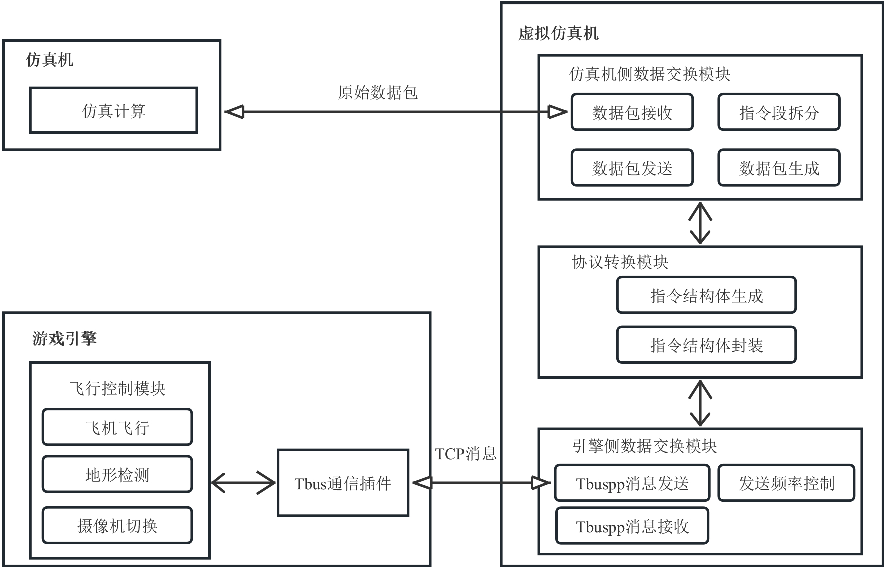
\includegraphics[width=\textwidth]{pictures/framework.pdf}
        \caption{数据交换子系统架构图}
        \label{subframe}
    \end{center}
\end{figure}
\subsection{系统逻辑视图}
逻辑视图以用户为中心,展示了系统的架构和功能模块。系统通过逻辑层次划分,把各个功能抽象成类,实现功能的封装。
如图\ref{logic}描述了系统的逻辑视图。SimNodeCommunicate代表仿真机与虚拟仿真机间沟通的模块,包含EstablishConnection功能,负责建立维持底层网络的连接,在此基础上实现原始数据包的收发;
SendDataFrame和ReceviceDataFrame负责维护各自的消息队列,并真正执行原始数据包的发送和接收任务,前者将数据包交给数据转换模块,后者则将收到的数据反馈给仿真机。
DataConverter表示数据转换模块。来自仿真机的消息会经历原始数据包到中间指令结构体再到ProtoBuffer协议数据段的变换过程,反馈消息则与之相反。
DataAnalysis负责原始数据包重新解释为指令结构体或将结构体添加头部信息封装为原始数据包,DataEncapsulate负责指令结构体与ProtoBuffer结构间的转换。
GameEngineCommunication表示虚拟仿真机与游戏引擎间沟通的模块,使用到了Tbuspp这一插件,EstablishConnection同样负责建立和维持Tbus节点的连接,在此基础上收发TCP数据段。
SendDataSegement和ReceviceDataSegement负责维护各自的消息队列,并真正执行数据段的发送和接收任务,前者将数据段交给游戏逻辑使用,后者将反馈信息给到数据转换模块逆向转换。
GameLogic模块负责飞行模拟的运行逻辑,其中FlightControl模块负责控制飞机位置和旋转姿态,也是最基本的飞行模拟要求。Camera模块负责确定飞行画面渲染的范围,第一人称视角只会跟随飞机运动,环绕视角可以在飞机为中心的球面上移动,自由视角则可以在场景中漫游。
DetectTerrain负责检测飞机低空飞行时其下方的地形信息,此信息会被反馈给仿真机处理。
\begin{figure}[h]
    \begin{center}
        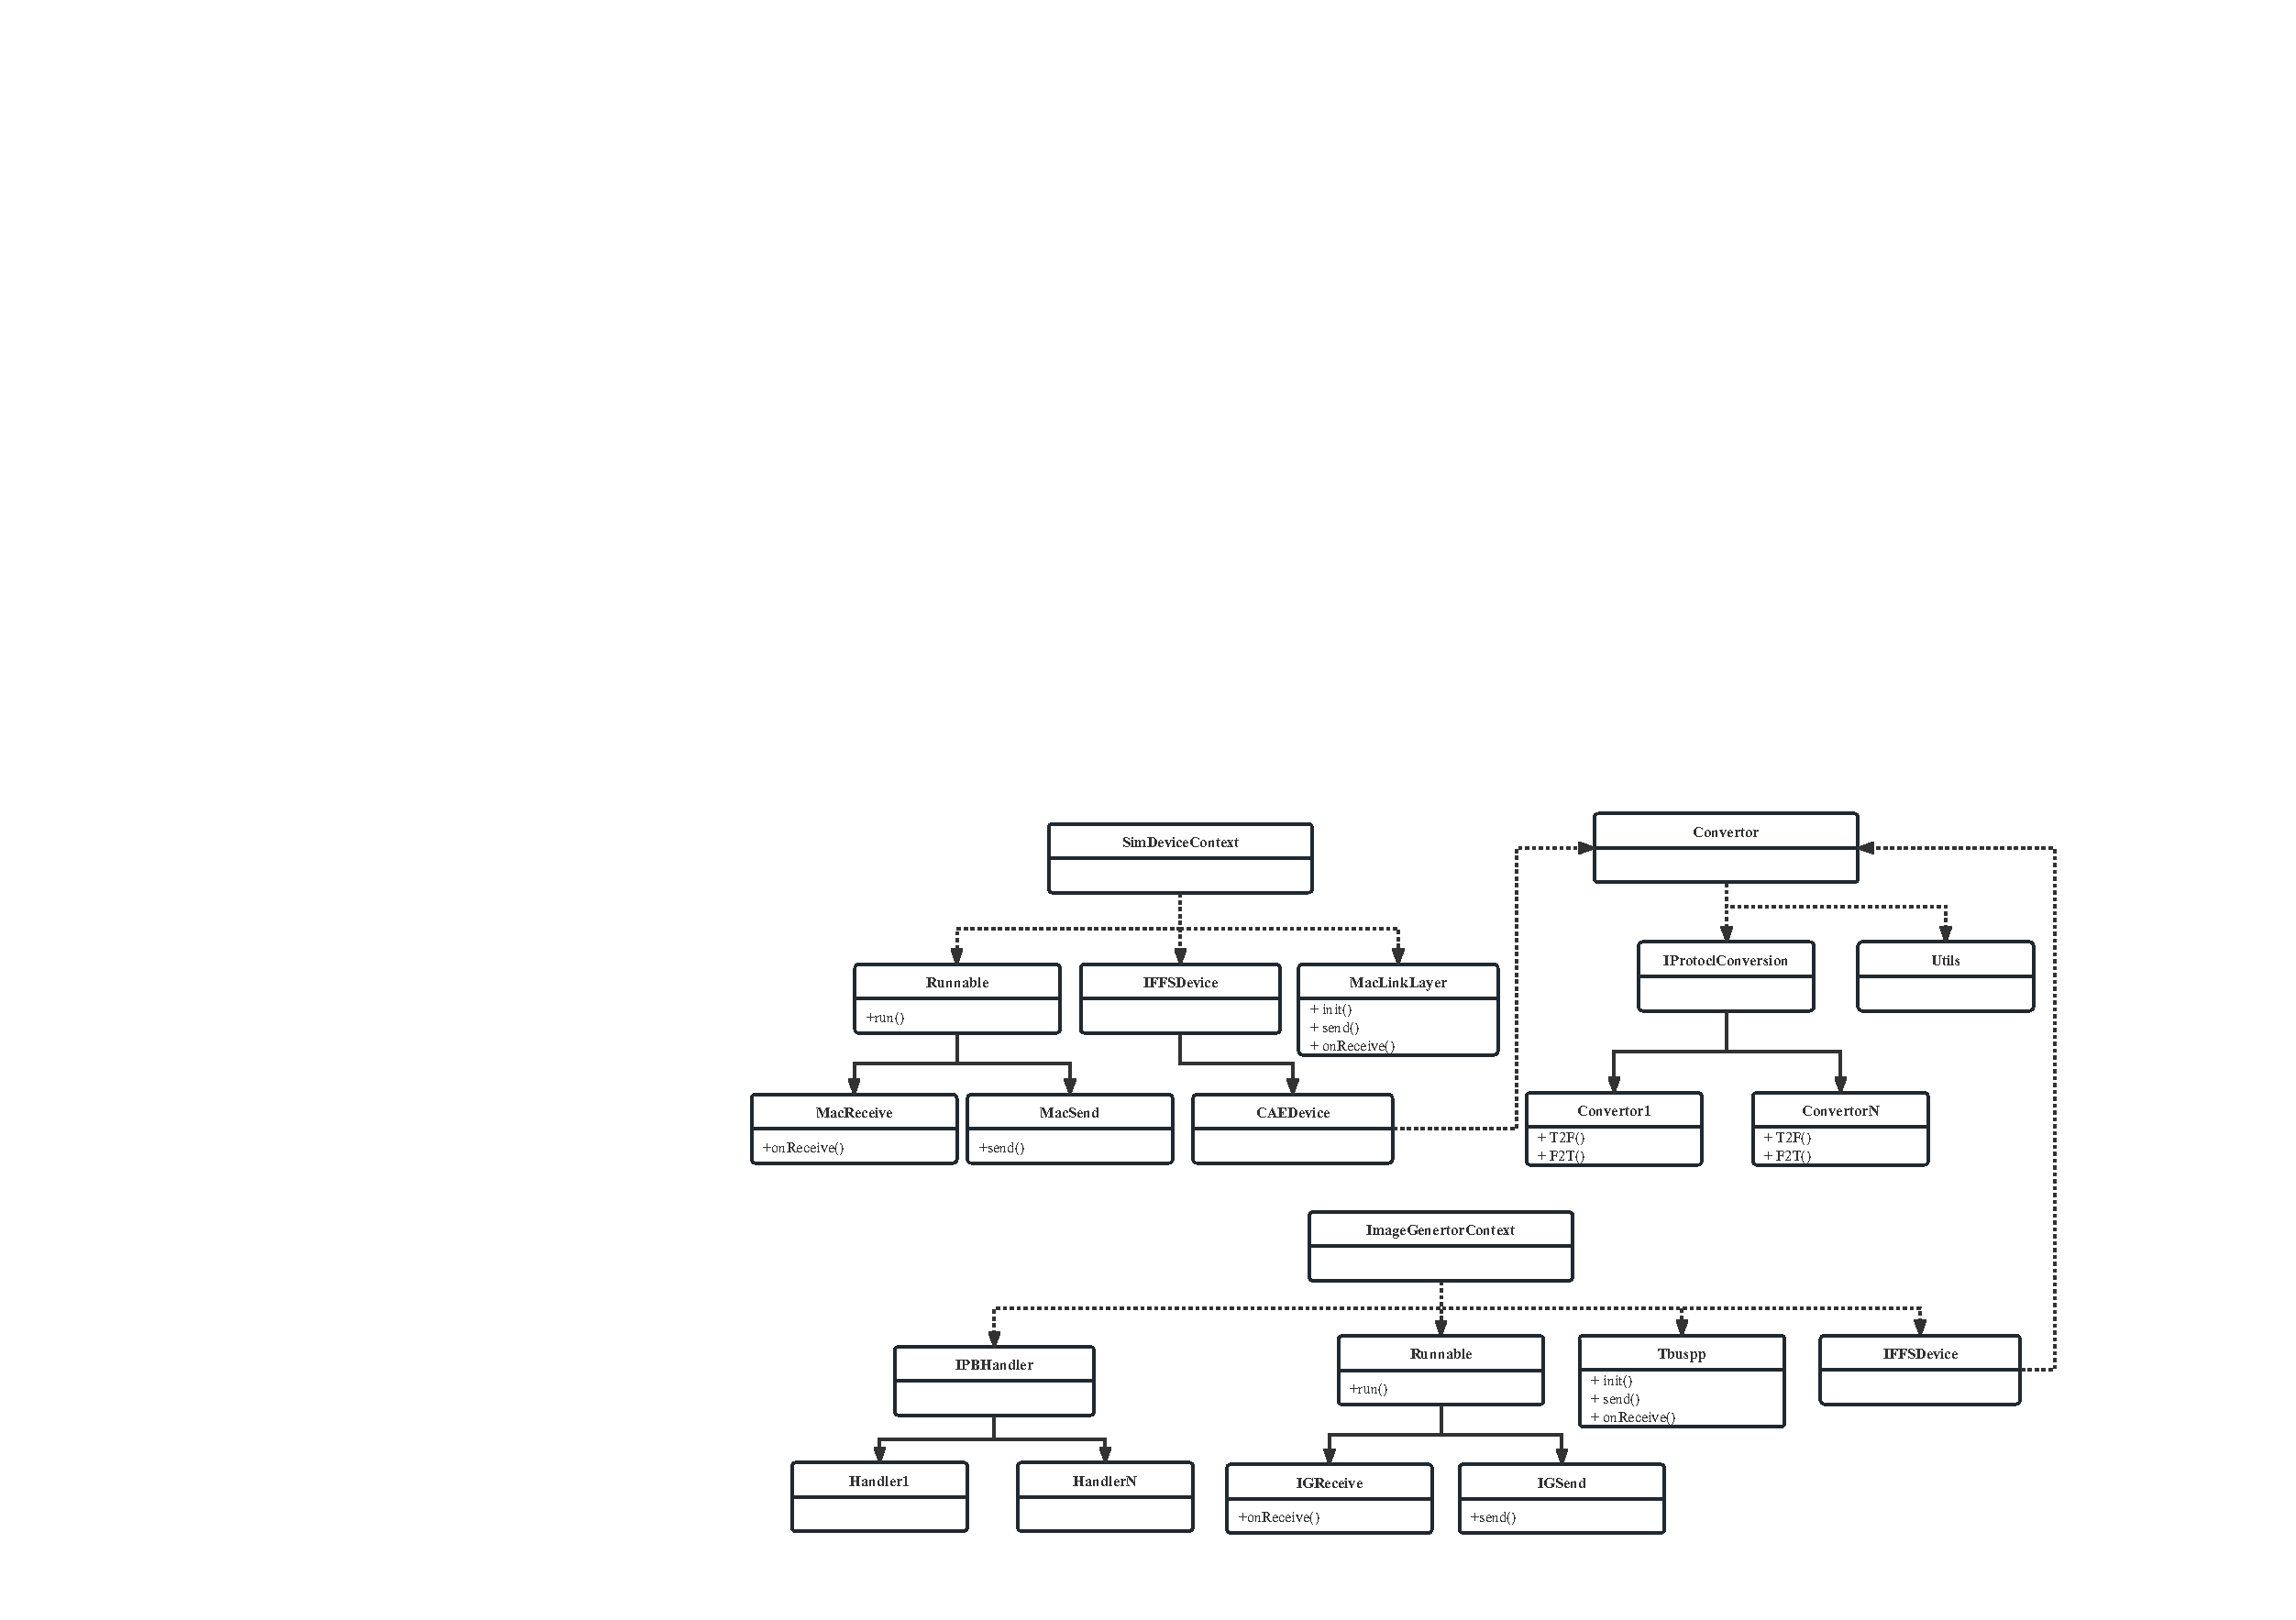
\includegraphics[width=\textwidth]{pictures/logic.pdf}
        \caption{逻辑视图}
        \label{logic}
    \end{center}
\end{figure}
\subsection{系统开发视图}
\begin{figure}[h]
    \begin{center}
        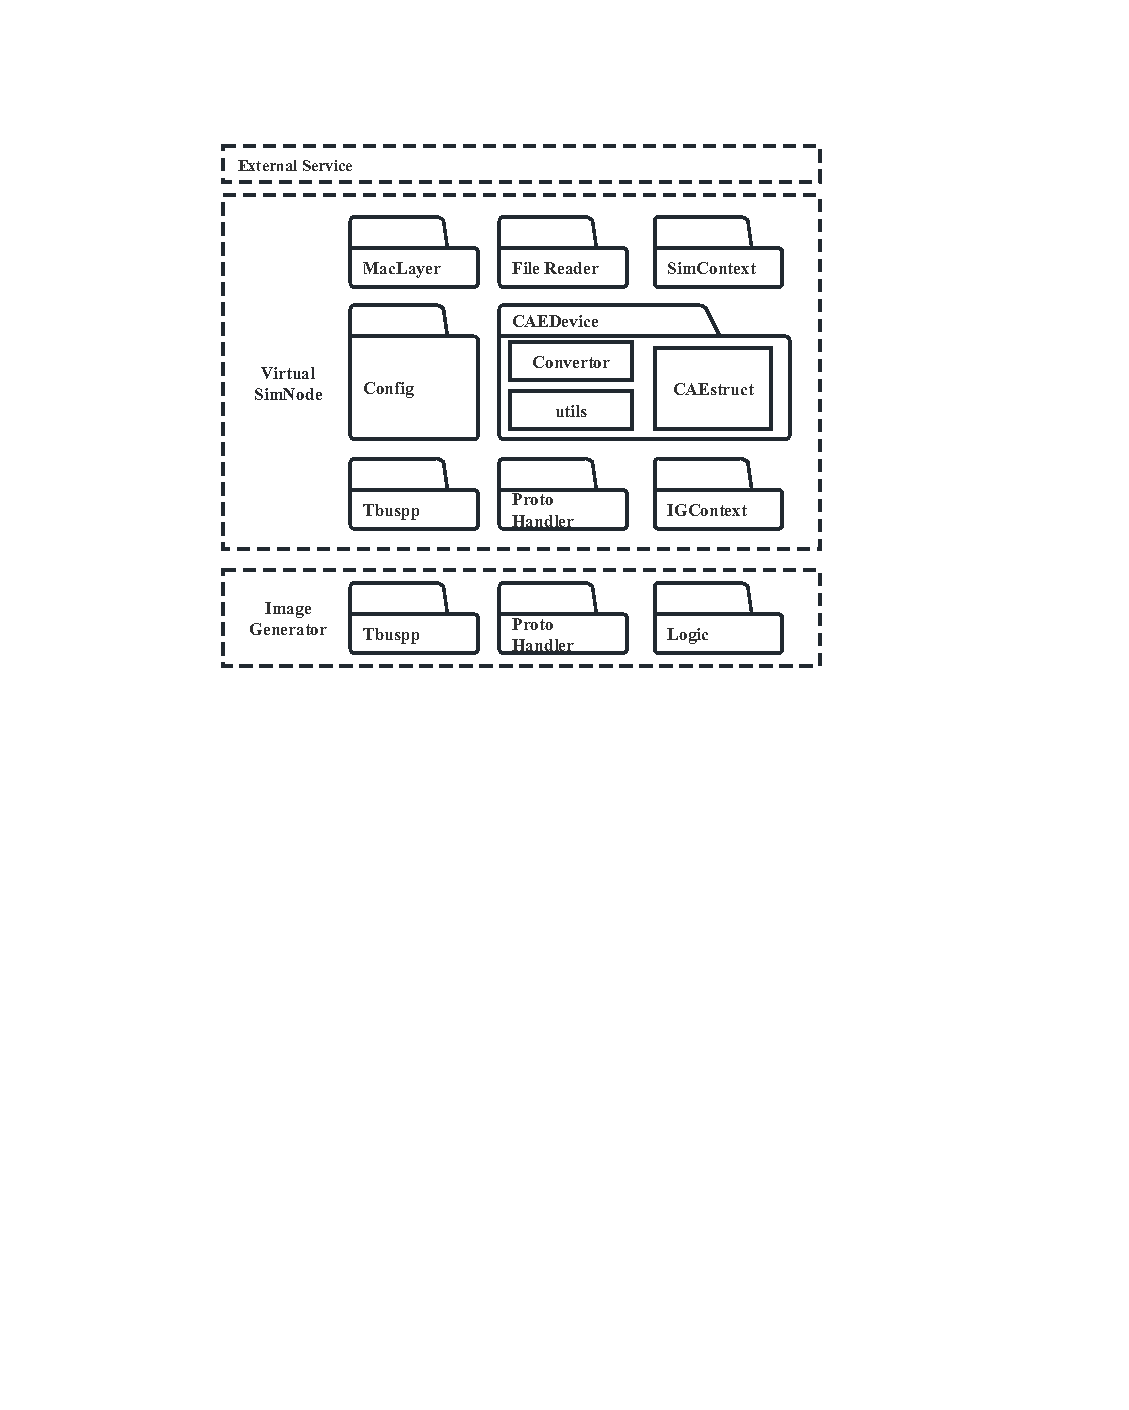
\includegraphics[width=0.8\textwidth]{pictures/devdiagram.pdf}
        \caption{开发视图}
        \label{dev}
    \end{center}
\end{figure}
\subsection{系统进程视图}
进程视图是用系统工程师的视角对系统进行阐述。可以详细阐述系统的动
态运行过程,重点描述系统运行时的行为。图\ref{procedure}是本系统的进程视图,
在虚拟仿真机中,主线程启动后会开启一个发送线程和一个接收线程,负责接收来自仿真机的数据处理后发送给游戏引擎,或者接收来自游戏引擎的反馈给到仿真机。
在游戏引擎中,逻辑线程负责接收到数据后完成对场景的布置,同时与发送线程同步,避免积累太多数据在内存中。逻辑线程同时需要计算碰撞情况并给出反馈信息。
渲染线程专门负责对逻辑线程中生成的场景进行渲染,一般来讲逻辑线程比渲染线程快一帧。

\begin{figure}[h]
    \begin{center}
        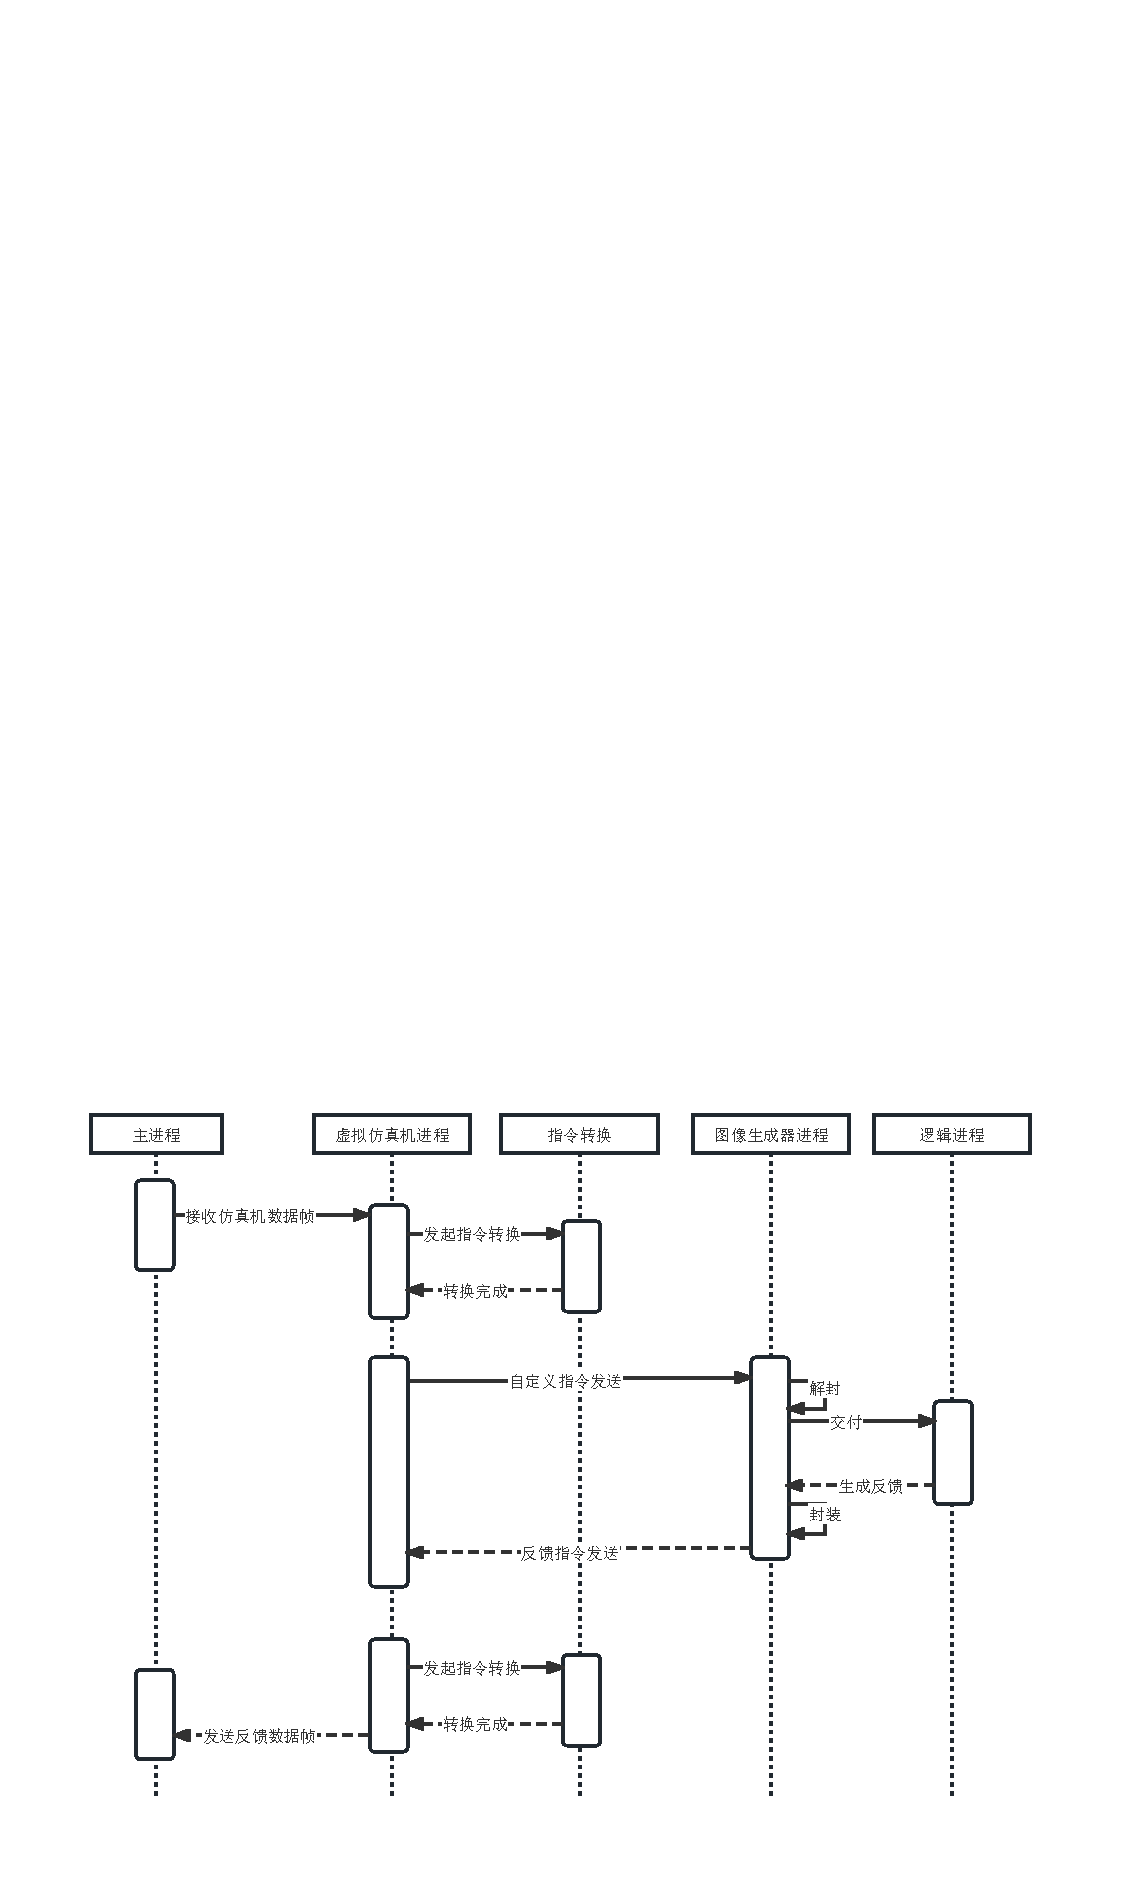
\includegraphics[width=0.8\textwidth]{pictures/procedure.pdf}
        \caption{进程视图}
        \label{procedure}
    \end{center} 
\end{figure}
\subsection{系统部署视图}
部署视图是用运维人员的视角对系统进行阐释。它着重于解释说明系
统的整体物理结构,包括各组件之间的连接方式等等,又称为物理视图。图\ref{deploydiagram}是本系
统的部署视图。飞行员在机舱中操作被仿真机记录并进行仿真计算,数据的解析和转换在虚拟仿真机内完成,游戏引擎收到TCP消息后完成场景的生成和渲染。
\begin{figure}[h]
    \begin{center}
        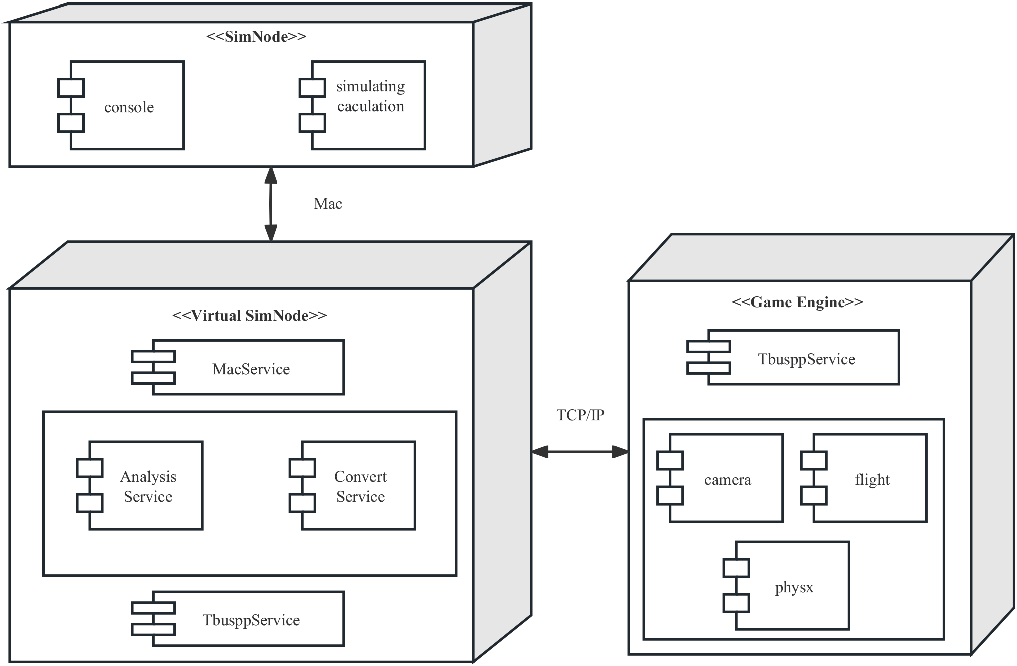
\includegraphics[width=0.8\textwidth]{pictures/deploydiagram.pdf}
        \caption{部署视图}
        \label{deploydiagram}
    \end{center}
\end{figure}
\section{数据交换子系统详细设计}
\subsection{仿真机侧数据交互模块}
仿真机侧数据交换模块负责虚拟仿真机与仿真机之间的交流。他们之间通过数据链路层的原始数据包进行沟通,即除去真实数据外,仅含有Mac地址等信息。因此不能依靠TCP/IP协议收发而是直接访问底层网络。
该模块会将到来的数据帧拆为指令结构体供后续使用,或者将指令结构体包装为数据帧发送给仿真机。
\par
本模块的主要执行流程如图\ref{module11}所示。流程分为接收消息和发送反馈消息两部分。在接收到消息后,需要先读取数据帧中的指令代号信息,如果代号已知,则调取对应的转换对象,将其中信息重新解释为对应的指令结构体。
由于指令代号有接近百种,项目初期只用到部分指令,对于未知的指令进行抛弃。发送反馈消息过程中,则需要对指令结构体添加数据帧头部信息,并通过底层网络直接发送。

\begin{figure}[h!]
    \begin{center}
        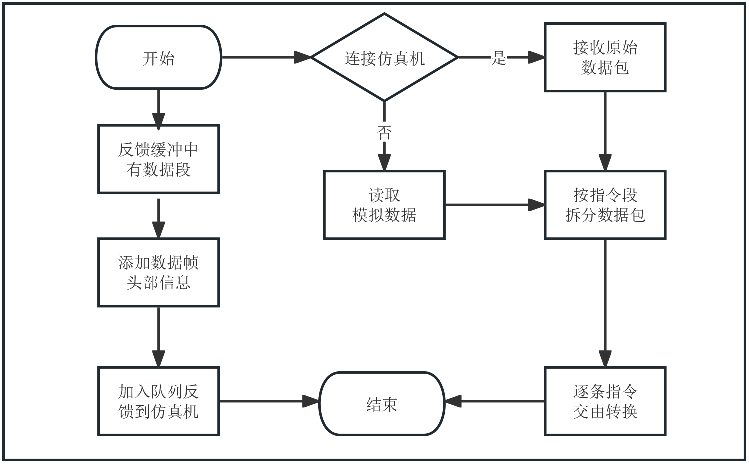
\includegraphics[width=0.8\textwidth]{pictures/flowchart1.pdf}
        \caption{仿真机侧数据交互流程图}
        \label{module11}
    \end{center}
\end{figure}
\par
本模块的核心类图如图\ref{module12}所示。其中的核心是类SimulationDeviceContext,它表示在虚拟仿真机中与仿真机交流的环境,其中包含控制信息收发的线程和待发送信息队列。
ISimulatorDeviceInterface则是与仿真机交流的接口,其中包含了对于数据帧中指令代号的读取方法GetSimOperateCode,以及发送消息给仿真机SendToSimulationDevice方法。
FullFightSimulatorDeviceBase中包含对该接口的实现。CAEGenericSimulatorDeviceBase代表CAE公司FFS设备,其中含有解读并转换该设备原始数据包的具体算法。当需要接入其他公司设备时,
只需要重新设计对应方法即可。
MacLinkCommunication类负责建立数据链路层连接并与真实仿真机进行原始数据包的交流。
\begin{figure}[h!]
    \begin{center}
        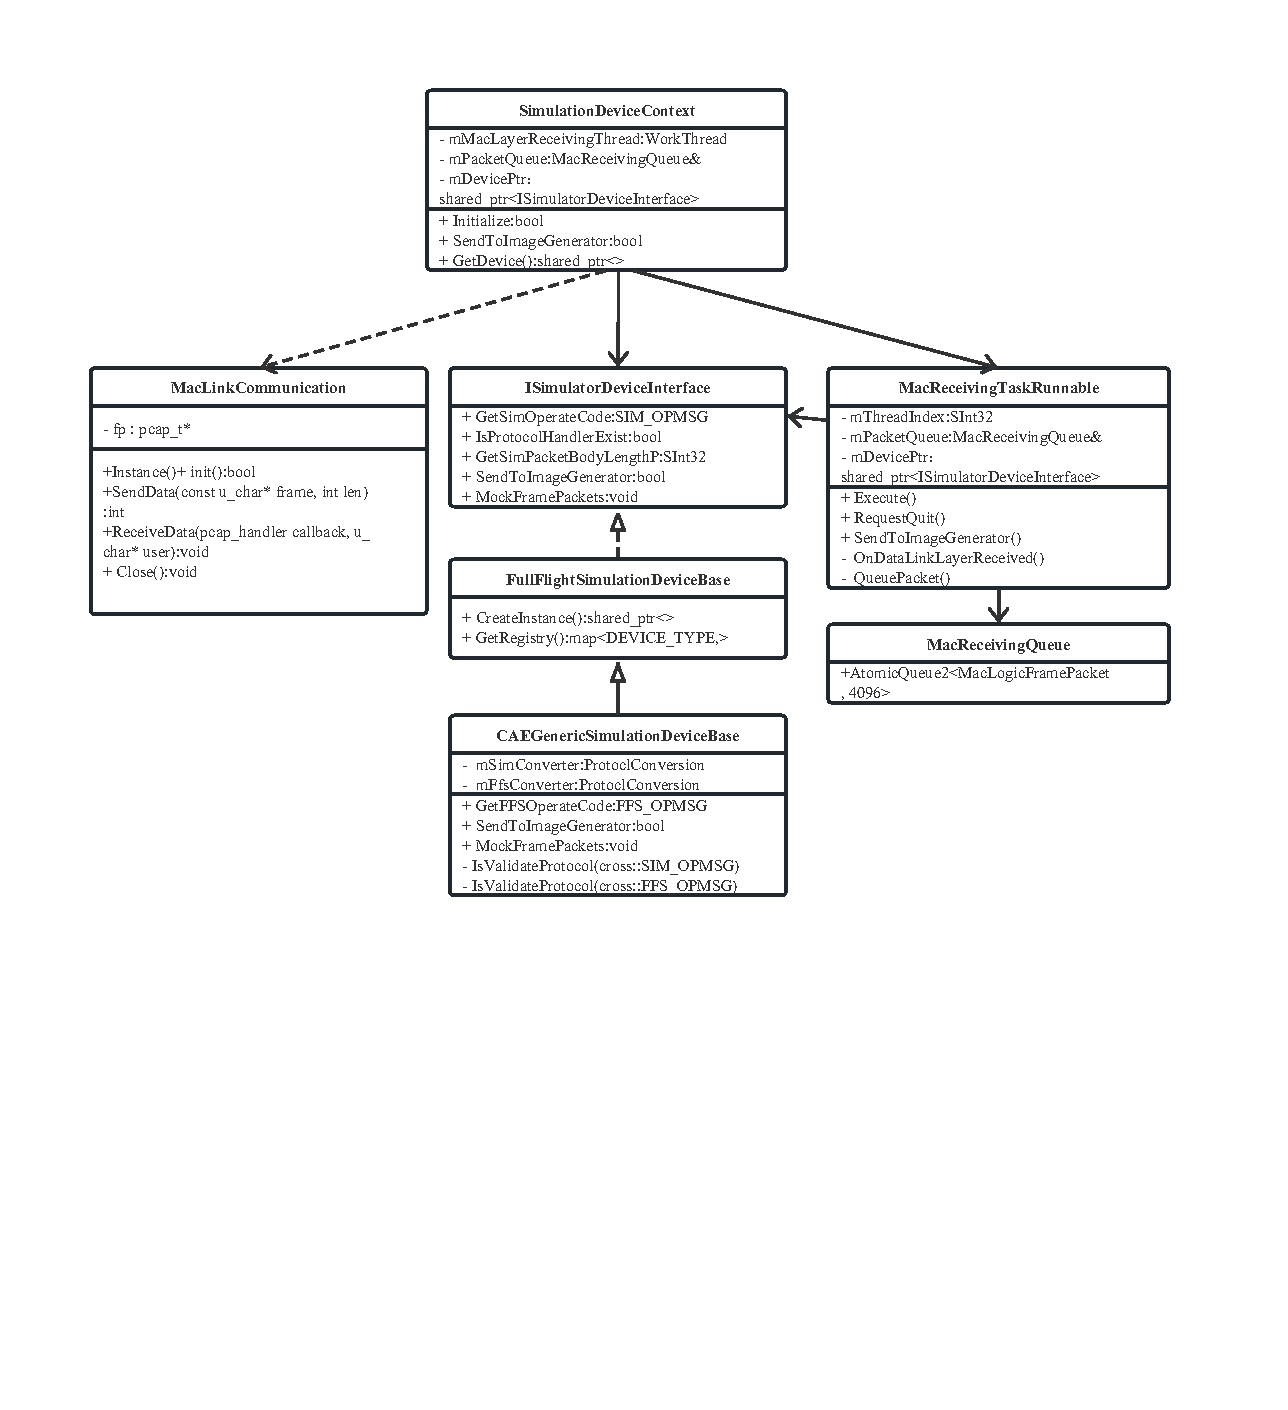
\includegraphics[width=\textwidth]{pictures/classdiagram1.pdf}
        \caption{仿真机侧数据交互核心类图}
        \label{module12}
    \end{center}
\end{figure}

\subsection{数据转换模块}
协议转换模块负责指令结构体与ProtoBuffer协议结构间的封装与解封。从仿真机收到的消息中对于浮点数的表达方式是由该厂商自行设计的,对于不同精度要求的数据表示方式也存在差异。
因此这两种结构之间的转换需要严格依照设计文档中的说明设计转换算法,而不是简单的赋值。ProtoBuffer协议结构为给到游戏引擎的数据结构,指令结构体则是准备反馈给仿真机的结构。
\par
本模块的主要执行流程如图\ref{module21}所示。在封装的过程中,需要先确定该指令对应的ProtoBuffer结构,经过数据转换算法后得到该结构,之后添加部分头部信息便可将其加入发送队列。
解封时现根据头部信息确定指令类型,再使用逆向的数据转换算法生成指令结构体即可准备发送给仿真机。

\begin{figure}[h!]
    \begin{center}
        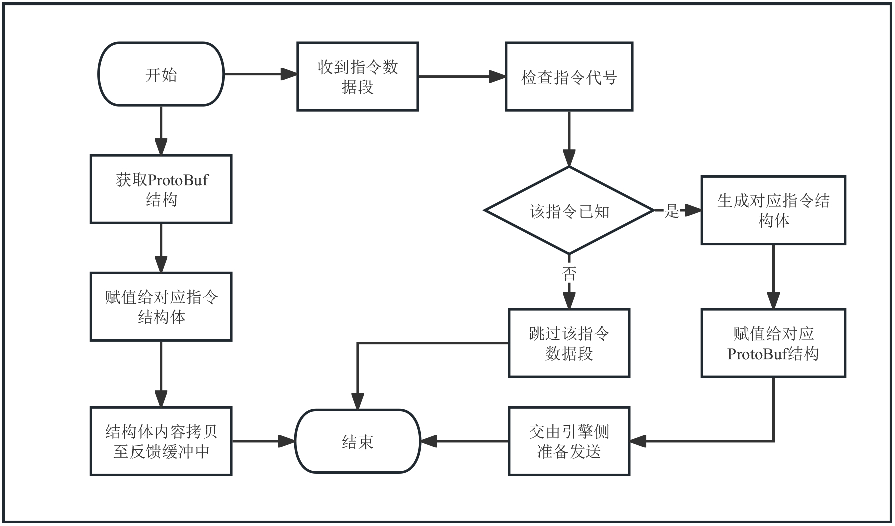
\includegraphics[width=0.8\textwidth]{pictures/flowchart2.pdf}
        \caption{数据转换流程图}
        \label{module21}
    \end{center}
\end{figure}
\par
本模块的核心类图如图\ref{module22}所示。其中核心为IProtoclConversion接口,其中声明了指令结构体与ProtoBuffer协议结构体互相转换的两种方法Convert。
ProtoclConversion是一个模板类,成员属性T表示一个指令结构体,成员属性F表示一个ProtoBuffer协议结构体,T和F组成互相转换的一对。该模板实例化的对象调用Convert方法便可以调用到对应结构体的转换方法。
SD\_PACKET\_21H是一个指令结构体的实例类型,包含了经纬度欧拉角等飞机飞行信息,其中也含有该指令类型转换的具体方法,发送给仿真机的队列MacLogicFramePacket由添加了数据帧头的指令结构体构成。
GeodeticCSUpdateStruct为SD\_PACKET\_21H指令结构体对应的ProtoBuffer协议结构体,发送给游戏引擎的消息队列FfsLogicFramePacket由各种ProtoBuffer协议结构体组成。

\begin{figure}[h!]
    \begin{center}
        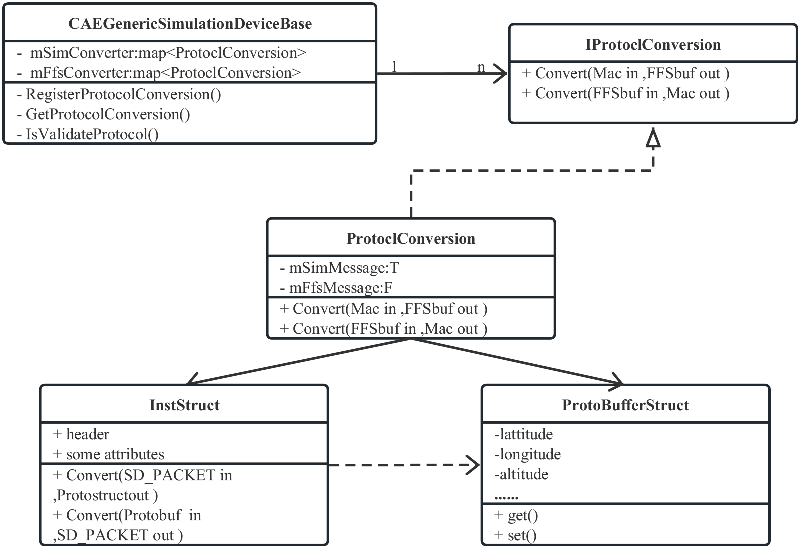
\includegraphics[width=\textwidth]{pictures/classdiagram2.pdf}
        \caption{数据转换核心类图}
        \label{module22}
    \end{center}
\end{figure}
\subsection{图像生成器侧数据交互模块}
游戏引擎侧数据交换模块负责虚拟仿真机与游戏引擎之间的交流。其利用Tbuspp插件使用TCP消息沟通,数据交换协议则是ProtoBuffer。再发送给游戏引擎的过程中,需要将发送频率的固定,因此该线程会以固定的频率被唤醒。
\par
本模块的主要执行流程如图\ref{module31}所示。当发送队列中有消息时,若可以进行发送则直接发送,否则要等待新的发送时机。反馈消息接收时则不需考虑频率,直接接收消息并给到协议转换模块。
\begin{figure}[h!]
    \begin{center}
        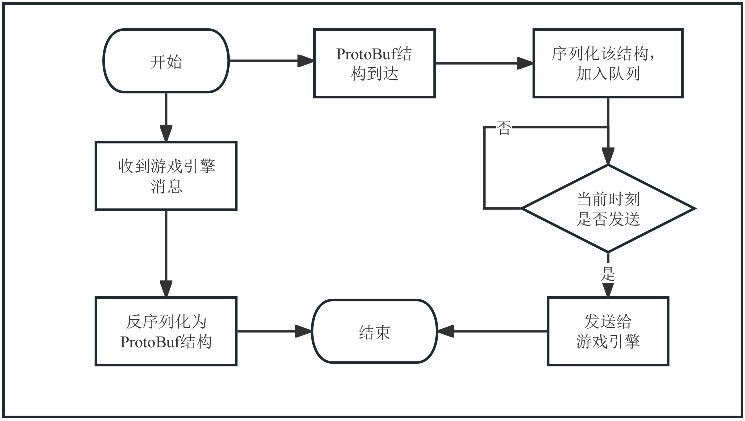
\includegraphics[width=0.8\textwidth]{pictures/flowchart3.pdf}
        \caption{视景系统侧数据交互流程图}
        \label{module31}
    \end{center}
\end{figure}
\par
本模块的核心类图如图\ref{module32}所示。其中的核心是类ImageGeneratorContext,它表示在虚拟仿真机中与游戏引擎交流的环境,其中包含控制信息收发的线程和信息队列。
IImageGeneratorDeviceInterface则是与游戏引擎交流的接口,其中包含了对于ProtoBuffer结构中指令代号的读取方法GetOperateCode,以及发送消息给游戏引擎SendToImageGenerator方法。
FullFightSimulatorDeviceBase是对该接口的实现,其依赖控制发送频率的类FrameSynchronization。CAEGenericSimulatorDeviceBase代表CAE公司FFS设备,其中含有与该公司设备进行沟通的具体方法。
\begin{figure}[h!]
    \begin{center}
        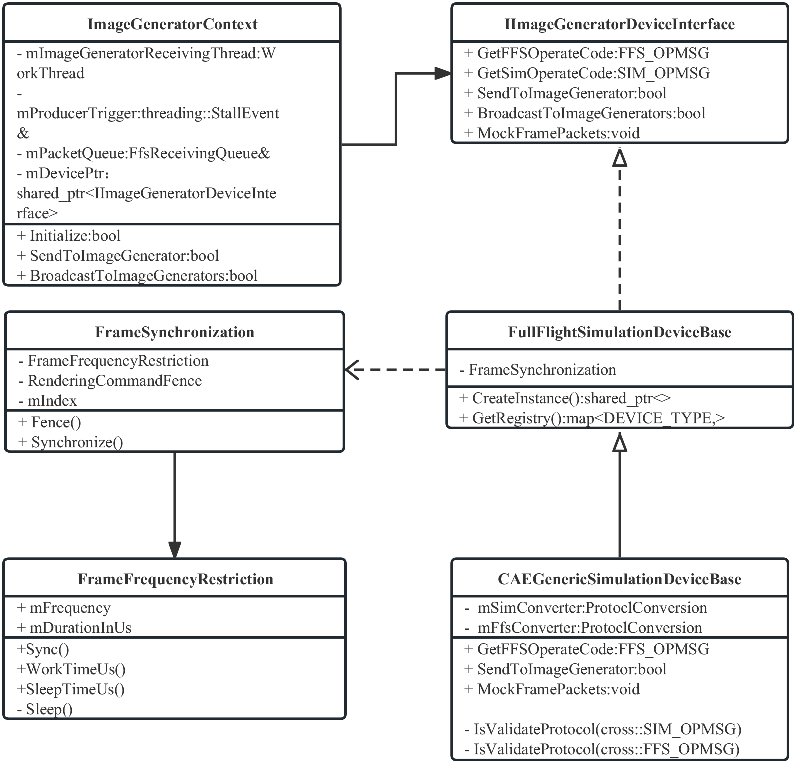
\includegraphics[width=\textwidth]{pictures/classdiagram3.pdf}
        \caption{视景系统侧数据交互核心类图}
        \label{module32}
    \end{center}
\end{figure}
\subsection{数据同步模块}
\subsection{飞行数据处理模块}
基础飞行控制模块负责让视景系统中的飞机运动起来并能被开发人员细致观察。实际过程中,游戏引擎会根据接收的数据实时改变飞机位置和飞行姿态,并加载周边场景信息。
飞机会随时对当前竖直下方的地形信息进行探测,并作为反馈信息。飞行过程中开发人员可以进行三种视角的观察。
\par
本模块的主要执行流程如图\ref{module41}所示。对于不用于飞机位置的指令直接跳过。对于位置和姿态信息则需要一定的转换,因为其在指令中的定义与场景是不同的坐标系。数据经过转换后便可以直接给到飞机实体和摄像机,改变其在场景中的位置,生成连贯的飞行画面。
\par
本模块的核心类图如图\ref{module42}所示。其中用于飞机位置控制的类为TransformSystemG,这是位于游戏引擎核心中的一个类,负责控制场景中实体的位置和旋转。其中列出了与球面世界相关的函数,主要为WGS84,ECFC和东北天三种坐标系的相互转换方法。
ControllabeUnit类可以给场景中的实体赋予被用户输入操作的能力,ControllableCamera继承自该类,其中含有RotationScale和TranslateScale属性调整移动和旋转的速度。
TestEnvControllableCamera则是为此视景系统专门定制的可控摄像机类,它可以在被控制的基础上实现三种控制模式间切换的功能。视景系统中的世界World需要依赖以上两个组件,实现飞机的飞行控制和摄像机的观察。
\begin{figure}[h!]
    \begin{center}
        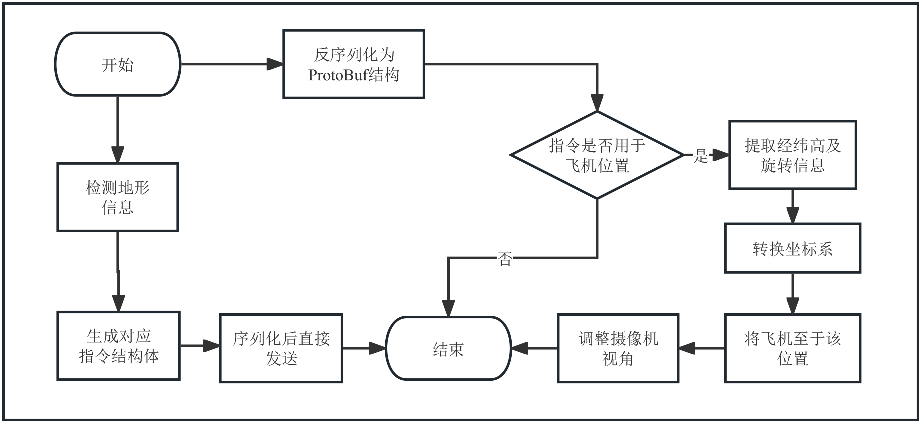
\includegraphics[width=0.8\textwidth]{pictures/flowchart4.pdf}
        \caption{飞行数据处理流程图}
        \label{module41}
    \end{center}
\end{figure}
\begin{figure}[h!]
    \begin{center}
        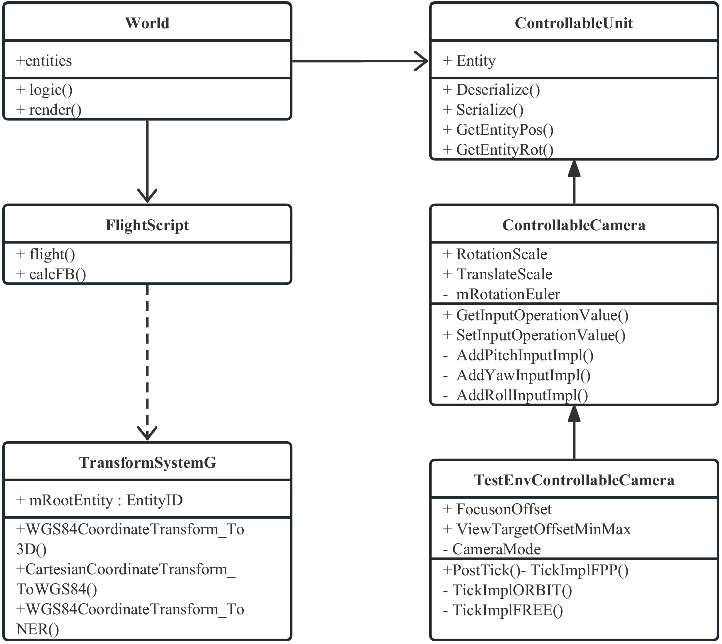
\includegraphics[width=\textwidth]{pictures/classdiagram4.pdf}
        \caption{飞行数据处理核心类图}
        \label{module42}
    \end{center}
\end{figure}
\section{本章小结}
按照软件开发的一般步骤,本章详细介绍了视景系统中数据交换子系统
的需求分析与设计过程。首先,对于整个视景系统的工作流程给出了整体说明。
其后,对数据交换子系统进行了需求分析,明确功能性需求和非功能性需求,
并以用例图和用例描述表的形式给出规格说明。其次,本章给出了数据交换子系统的架构设计。
最后,本章将子系统的主要功能划分为仿真机侧数据交换模块、协议转换模块、游戏引擎侧数据交换模块和基础飞行控制模块,
以流程图和核心类图描述了对各个模块的详细设计。